\chapter{Gabor Boosting Binary Classification}
\label{ch:bin}

\section{Gabor Wavelet and AdaBoost on Face Verification}
\label{sec:faceveri}
\subsection{Face Verification}
\paragraph{Inspiration}
\subsection{Gabor Wavelet}
\label{sec:faceveri:gabor}
\subsubsection{Gabor Wavelet Introduction}
A two-dimensional Gabor filter is a linear filter whose kernel is similar to the two-dimensional (2-D) receptive profiles of the mammalian cortical simple cells\cite{}. A 2-D Gabor kernel is a 2-D Gaussian function multiplied by a 2-D harmonic function. A harmonic function generally is Fourier basis function. Especially in a 2-D Gabor kernel, it is a sinusoidally modulated function, somewhere in a form of complex exponential function. The Gaussian function varies in dilation and the harmonic function varies in rotations, so that a group of 2-D Gabor filters can be formed into 2-D Gabor wavelets. Gabor wavelet can facilitates detection and recognition without correspondence, because it captures local structure corresponding to spatial frequency i.e. scale, spatial localisation i.e. coordinate, and orientation selectivity.
\subsubsection{Gabor Wavelet Background}
Gabor wavelet is modeled well as the receptive field profiles of cortical simple cells\cite{}. 2-D Gabor wavelet is widely adopted as a feature extraction approach in texture segmentation, iris recognition, face recognition, face expression recognition and so on. 

The problem of selecting the appropriate Gabor filters i.e. parameters characterised Gabor filters has been studied extensively and different classes of schemes have emerged. In \cite{Dunn1994}, 2-D Gabor filters transform different texture into detectable filter-output discontinuities at texture boundaries. Gabor filter output can be modeled as Rician random variables. A decision algorithm for selecting optimal filter parameters based on the Rician model developed by Dunn and Higgins\cite{Dunn1995}. In \cite{Jain1991}, a bank of Gabor filters are characterised as uniformly covering the spatial-frequency domain. A filter selection scheme is present based on minimal ``energy'' loss of reconstructed images from the filtered images. Teuner et al\cite{} choose parameters of Gabor filters based on the analysis of spectral feature contrasts obtained from iterations of pyramidal Gabor transforms. The benefit of the work is unnecessary to require a prior knowledge of the texture image so that the segmentation processing is unsupervised. Since these parametrisation solutions are all to choose optimal frequency or orientation of Gabor filter, an alternative wavelet scenario is proposed to bypass the optimisation. 

2-D Gabor wavelet model with multi-scale and multi-orientation was originally proposed by Daugman\cite{Daugman1985, Daugman1988} into biometric research. In \cite{Daugman1988}, by using a three-lay neural network, a nonorthogonal 2-D Gabor representation is generalised. Daugman also applied him 2-D Gabor wavelet model on human iris recognition.  In \cite{Daugman1993}, the visible texture of a person's iris is transformed into a sequence of multi-scale 2-D Gabor wavelet digits. Lades et al\cite{Lades1993} applied Gabor wavelets for face recognition using the Dynamic Link Architecture (DLA) framework. The DLA started by computing Gabor wavelets, and then it performs a flexible template comparison between resulting image decompositions using graph-matching. Wiskott et al.\cite{Wiskott1997,Wiskott1999} have extended on DLA when they developed a Gabor wavelet based Elastic Bunch Graph Matching (EBGM) to label and recognise faces. Faces are represented by labelled graphs using Gabor wavelet transform. The labels graphs consist nodes and edges which are positioned by elastic bunch graph matching processing with comparing similarities. The testing was done on the FERET database\cite{Phillips2000} showing a high recognition rate for frontal face images. Liu and Wechsler\cite{Liu2002} applied the Enhanced Fisher linear discriminant Model (EFM) to an augmented Gabor feature vector derived from the Gabor wavelet representation of face images. Liu\cite{Liu2004} also presents a Gabor-based kernel Principal Component Analysis (PCA) method by integrating Gabor wavelet representation of face images and the kernel PCA for recognition.  Fan et al.\cite{Fan2004} combined Gabor wavelet and Linear Discriminate Analysis (LDA) as Gabor wavelet applied to generate feature vectors and Null space-based LDA performed simultaneously on each orientations. 

In analysis of facial expression, the recognition is to analyse the relationship between the movements made by facial features, such as eyebrows, eyes and mouth. These facial features can be defined as point-based visual properties of facial expressions. Hong et al.\cite{Hong1998} use Gabor wavelets of five frequencies and eight orientations to define a ``big'' General Face Knowledge (GFK) with 50 nodes on face, and a ``small'' 16-node GFK with three frequencies and four orientations. The method which fits these nodes with face image is the elastic graph matching proposed by Wiskott et al.\cite{Wiskott1997,Wiskott1999} in face recognition. Zhang et al.\cite{Zhang1998} use 34 facial points for which a set of Gabor wavelet coefficients, The Gabor wavelets with three frequencies and six orientations have been utilised. Lyons et al.\cite{Lyons1999} used a fiducial grid of 34 nodes and apply wavelets of five frequencies and six orientations.
\subsubsection{The Definition of Gabor Wavelet}
Gabor wavelets were introduced to image analysis due to their biological relevance and computational properties. A Gabor wavelet \cite{Daugman1988} (somewhere, called Gabor Kernel or Gabor Elemental Function\cite{Dunn1994}) is defined as 
\begin{equation}\label{eq:kernel}
   \psi_{\mu,\nu}(z)=\frac{\|{k_{\mu,\nu}}\| ^ {2}}{\sigma ^{2}}e^{-\frac{\|{k_{\mu,\nu}}\|^ {2}\|z\|^{2}}{2\sigma ^{2}}}\lbrack{e^{ik_{\mu,\nu} z}-e^{-\frac{\sigma^2}{2}}}\rbrack
\end{equation}
where $z=(x,y)$ indicates a point with $x$ i.e. the horizontal coordinate and $y$ i.e. the vertical coordinate. $\mu$ and $\nu$ define the angular orientation and the spatial frequencies of the Gabor kernels. Because the spatial frequency modulates the size of 2-D discrete Gabor kernel, $\nu$ also define as the scale of kernel. $\|\cdot\|$ denotes the norm operator. $\sigma$ is the standard derivation of Gaussian window in the kernel. The wave vector $k_{\mu,\nu}$ is defined as follows
\begin{equation}\label{eq:wavevector}
k_{\mu,\nu}=k_{\nu}e^{i\phi_{\mu}}
\end{equation}
where $k_{\nu}=\frac{k_{max}}{f^{\nu}}$ and $\phi_{\mu}=\frac{\pi\mu}{8}$ if eight different orientations have been chosen. $k_{max}$ is the maximum frequency, and $f$ is the spatial factor between
kernels in the frequency domain.
\paragraph{Why becomes Wavelets}
The Gabor kernels in \mbox{Equation} (\ref{eq:kernel}) are all self-similar since they can be generated from one kernel (a mother wavelet) by dilation and rotation via the wave vector $k_{\mu,\nu}$. Each kernel is a product of a Gaussian envelope
\begin{equation}\label{eq:gaussian}
 \frac{\|{k_{\mu,\nu}}\| ^ {2}}{\sigma ^{2}}e^{-\frac{\|{k_{\mu,\nu}}\|^ {2}\|z\|^{2}}{2\sigma ^{2}}}\
\end{equation}
and a complex plane wave $e^{ik_{\mu,\nu} z}$. The complex wave determines the oscillatory part of the kernel. $-e^{-\frac{\sigma^2}{2}}$ compensates for the DC value, which makes the kernel DC-free. DC-free \cite{Krueger2001} is a wavelet term that means wavelets do not lose any generality or minimal energy loss when images are reconstructed by the wavelets. The effect of the DC term becomes negligible when the parameter $\sigma$, which determines the ratio of the Gaussian window width to wavelength, is a sufficiently large value.

In the thesis, five different scales and eight orientations of Gabor wavelets are used, i.e., $\nu\in\{-1,\ldots,3\}$, and $\mu\in\{0,\ldots,7\}$, The images adopted are smaller than the images used in \cite{}, so that the scale range is from $-1$ to $3$ rather than from $0$ to $4$ in previous work. The eight orientations in radian are $0$, $\pi/8$, $\pi/4$, $3\pi/8$, $\pi/2$, $5\pi/8$, $3\pi/4$, and $7\pi/8$. Gabor wavelets are restricted by a Gaussian envelope function with relative width $\sigma=2\pi$ according. The maximum frequency is $k_{max}=\frac{\pi}{2}$, and the factor $f=\sqrt{2}$. These parameters are chosen according to \cite{}. The kernels exhibit desirable characteristics of spatial frequency, spatial locality, and orientation selectivity. 

Since Gabor kernel is a product of a Gaussian and a complex plane wave. A complex mathamatic form consists real unit and imaginary unit, also called even and odd. To separate \ref{eq:kernel} into real and imaginary unit, so that the real part is
\begin{equation}\label{eq:real}
\frac{k_{\nu}^2}{\sigma^2}e^{-{\frac{\|z\|^2 k_{\nu}^2}{2\sigma^2}}} \{\cos(k_{\nu}\cos(\phi_{\mu})x+k_{\nu}\sin(\phi_{\mu})y)-e^-{\frac{\sigma^2}{2}}\}
\end{equation}
and the imaginary part becomes
\begin{equation}\label{eq:imag}
\frac{k_{\nu}^2}{\sigma^2} e^-{\frac{\|z\|^2 k_{\nu}^2}{2\sigma^2}} \sin(k_{\nu}\cos(\phi_{\mu})x+k_{\nu}\sin(\phi_{\mu})y)
\end{equation}
In the thesis, five scales and eight orientations are adopted, the real part of these 40 Gabor wavelets are shown in \mbox{Figure} \ref{fig:realgabor}. The imaginary part of these 40 Gabor wavelets are shown in \mbox{Figure} \ref{fig:imaggabor} 
\begin{figure}
 \begin{center}
 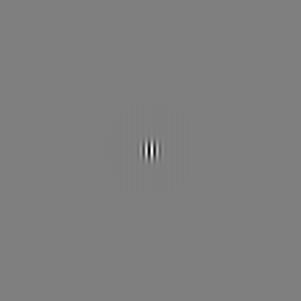
\includegraphics[scale=0.1]{ch4/figures/rGabor0_0.jpg}
 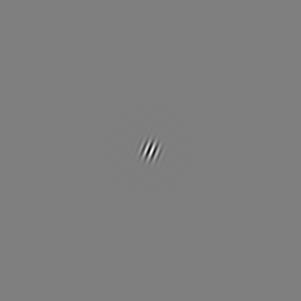
\includegraphics[scale=0.1]{ch4/figures/rGabor0_1.jpg}
 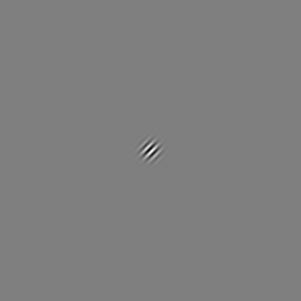
\includegraphics[scale=0.1]{ch4/figures/rGabor0_2.jpg}
 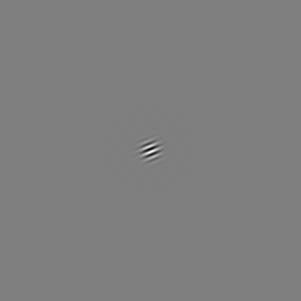
\includegraphics[scale=0.1]{ch4/figures/rGabor0_3.jpg}
 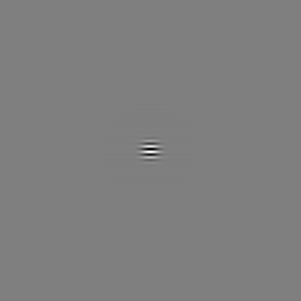
\includegraphics[scale=0.1]{ch4/figures/rGabor0_4.jpg}
 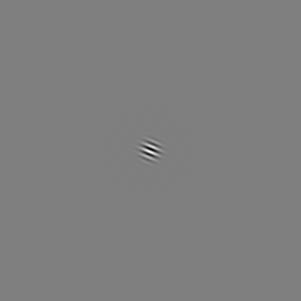
\includegraphics[scale=0.1]{ch4/figures/rGabor0_5.jpg}
 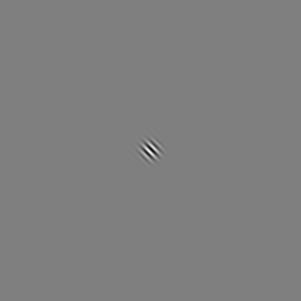
\includegraphics[scale=0.1]{ch4/figures/rGabor0_6.jpg}
 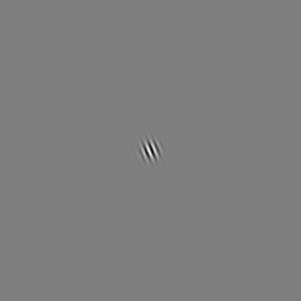
\includegraphics[scale=0.1]{ch4/figures/rGabor0_7.jpg}\\
 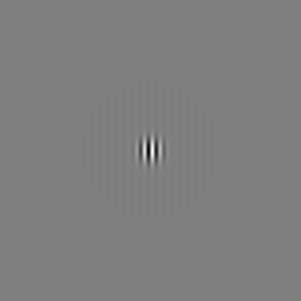
\includegraphics[scale=0.1]{ch4/figures/rGabor1_0.jpg}
 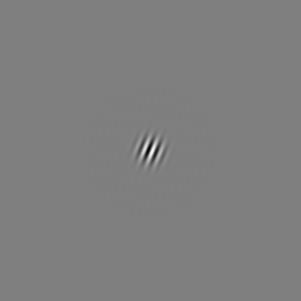
\includegraphics[scale=0.1]{ch4/figures/rGabor1_1.jpg}
 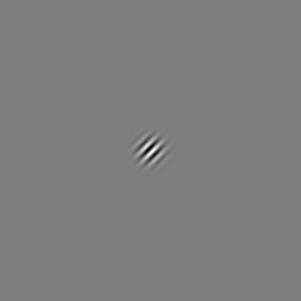
\includegraphics[scale=0.1]{ch4/figures/rGabor1_2.jpg}
 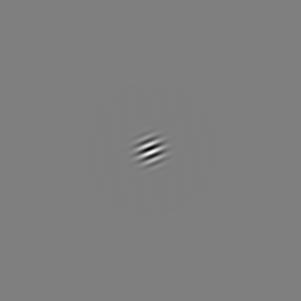
\includegraphics[scale=0.1]{ch4/figures/rGabor1_3.jpg}
 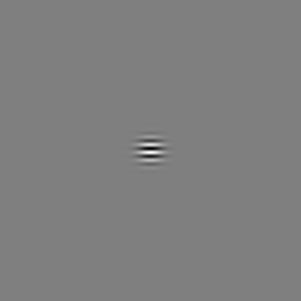
\includegraphics[scale=0.1]{ch4/figures/rGabor1_4.jpg}
 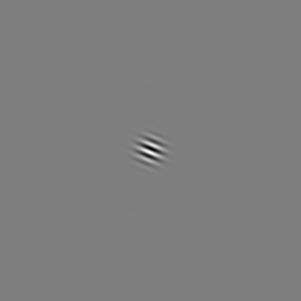
\includegraphics[scale=0.1]{ch4/figures/rGabor1_5.jpg}
 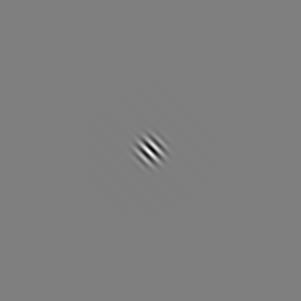
\includegraphics[scale=0.1]{ch4/figures/rGabor1_6.jpg}
 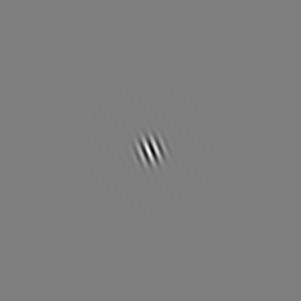
\includegraphics[scale=0.1]{ch4/figures/rGabor1_7.jpg}\\
 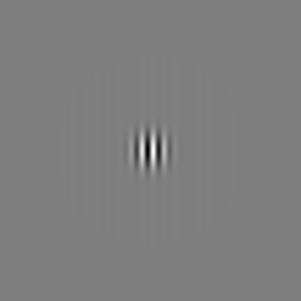
\includegraphics[scale=0.1]{ch4/figures/rGabor2_0.jpg}
 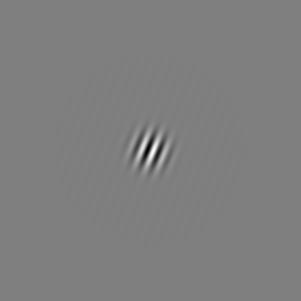
\includegraphics[scale=0.1]{ch4/figures/rGabor2_1.jpg}
 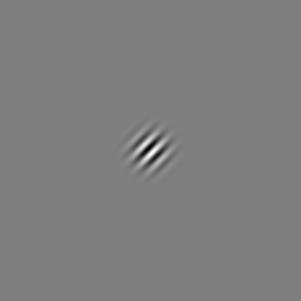
\includegraphics[scale=0.1]{ch4/figures/rGabor2_2.jpg}
 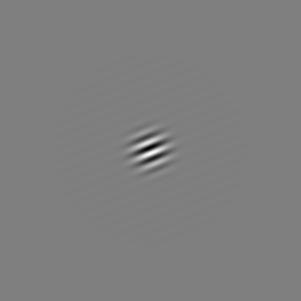
\includegraphics[scale=0.1]{ch4/figures/rGabor2_3.jpg}
 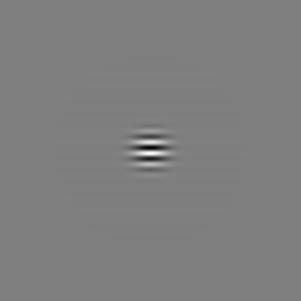
\includegraphics[scale=0.1]{ch4/figures/rGabor2_4.jpg}
 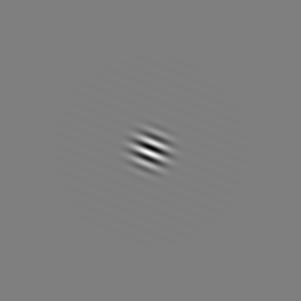
\includegraphics[scale=0.1]{ch4/figures/rGabor2_5.jpg}
 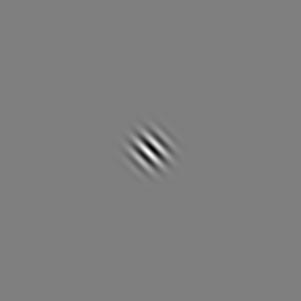
\includegraphics[scale=0.1]{ch4/figures/rGabor2_6.jpg}
 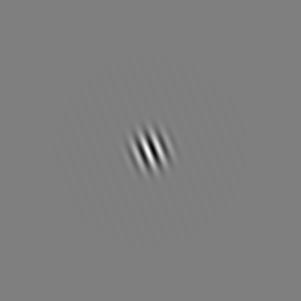
\includegraphics[scale=0.1]{ch4/figures/rGabor2_7.jpg}\\
 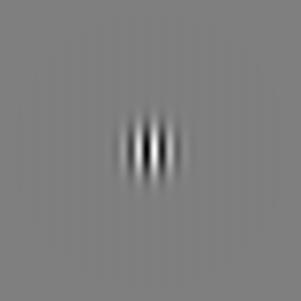
\includegraphics[scale=0.1]{ch4/figures/rGabor3_0.jpg}
 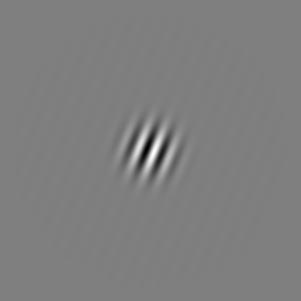
\includegraphics[scale=0.1]{ch4/figures/rGabor3_1.jpg}
 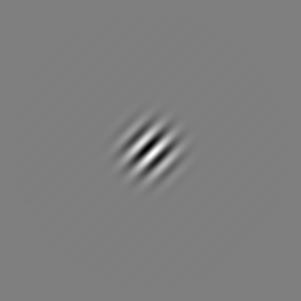
\includegraphics[scale=0.1]{ch4/figures/rGabor3_2.jpg}
 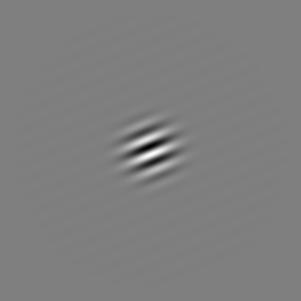
\includegraphics[scale=0.1]{ch4/figures/rGabor3_3.jpg}
 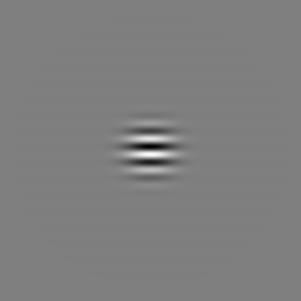
\includegraphics[scale=0.1]{ch4/figures/rGabor3_4.jpg}
 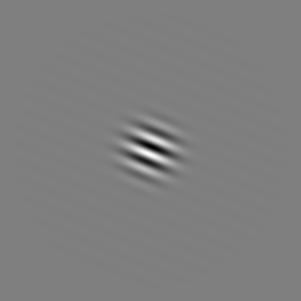
\includegraphics[scale=0.1]{ch4/figures/rGabor3_5.jpg}
 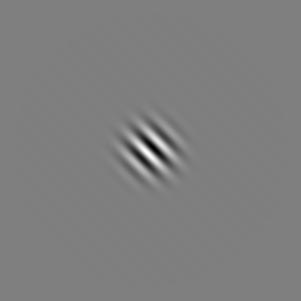
\includegraphics[scale=0.1]{ch4/figures/rGabor3_6.jpg}
 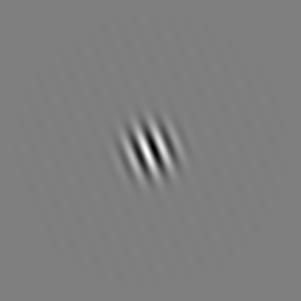
\includegraphics[scale=0.1]{ch4/figures/rGabor3_7.jpg}\\
 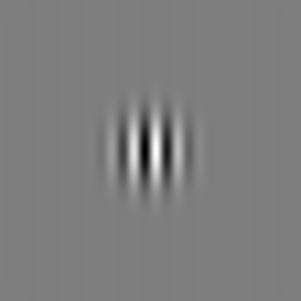
\includegraphics[scale=0.1]{ch4/figures/rGabor4_0.jpg}
 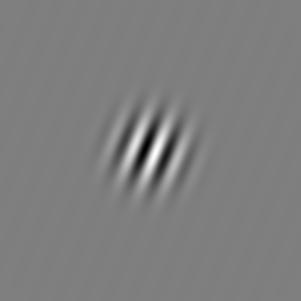
\includegraphics[scale=0.1]{ch4/figures/rGabor4_1.jpg}
 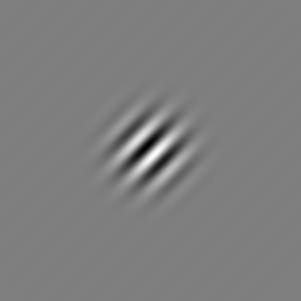
\includegraphics[scale=0.1]{ch4/figures/rGabor4_2.jpg}
 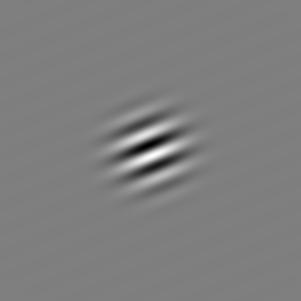
\includegraphics[scale=0.1]{ch4/figures/rGabor4_3.jpg}
 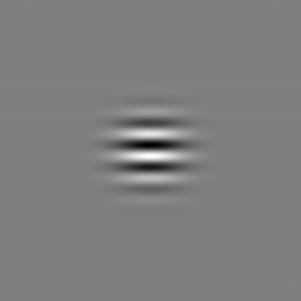
\includegraphics[scale=0.1]{ch4/figures/rGabor4_4.jpg}
 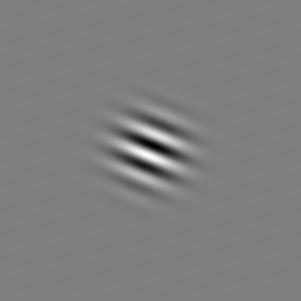
\includegraphics[scale=0.1]{ch4/figures/rGabor4_5.jpg}
 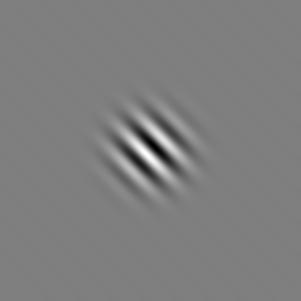
\includegraphics[scale=0.1]{ch4/figures/rGabor4_6.jpg}
 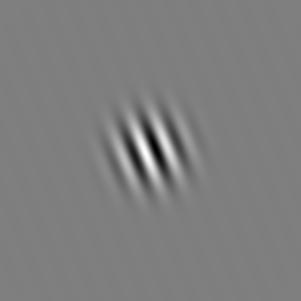
\includegraphics[scale=0.1]{ch4/figures/rGabor4_7.jpg}\\
 % RGabor.jpg: 1302x779 pixel, 72dpi, 45.93x27.48 cm, bb=0 0 1302 779
\end{center}
\caption{The real part of the $5\times8$ Gabor wavelets. These Gabor wavelets share 5 scales and 8 orientations. These orientations from left to right are $0,\frac{\pi}{8},\frac{\pi}{4},\frac{3\pi}{8},\frac{\pi}{2},\frac{5\pi}{8},\frac{3\pi}{4},$ and $\frac{7\pi}{8},$. The scales from top to bottom are $0$, $1$, $2$, $3$, $4$.}
\label{fig:realgabor}
\end{figure} 



\begin{figure}
 \begin{center}
 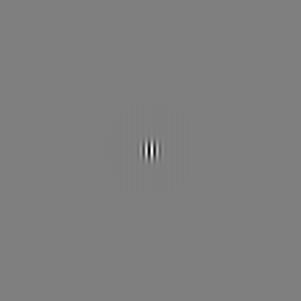
\includegraphics[scale=0.1]{ch4/figures/iGabor0_0.jpg}
 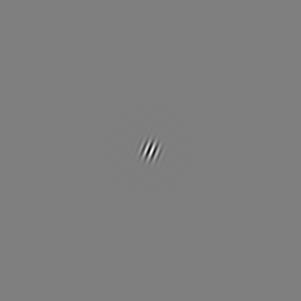
\includegraphics[scale=0.1]{ch4/figures/iGabor0_1.jpg}
 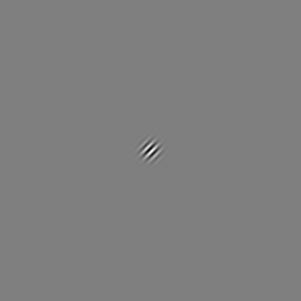
\includegraphics[scale=0.1]{ch4/figures/iGabor0_2.jpg}
 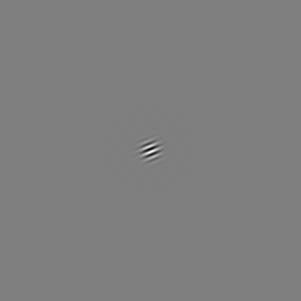
\includegraphics[scale=0.1]{ch4/figures/iGabor0_3.jpg}
 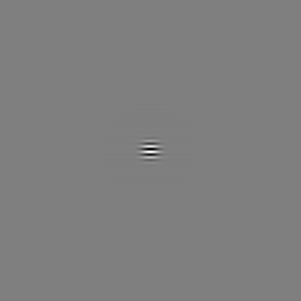
\includegraphics[scale=0.1]{ch4/figures/iGabor0_4.jpg}
 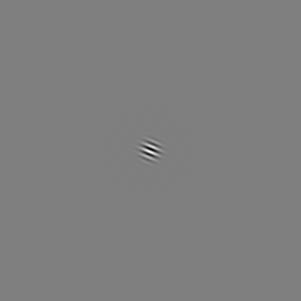
\includegraphics[scale=0.1]{ch4/figures/iGabor0_5.jpg}
 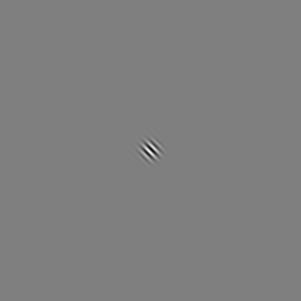
\includegraphics[scale=0.1]{ch4/figures/iGabor0_6.jpg}
 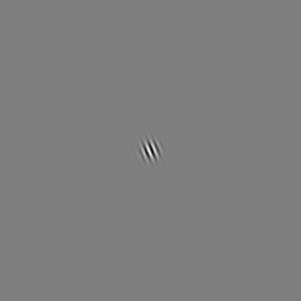
\includegraphics[scale=0.1]{ch4/figures/iGabor0_7.jpg}\\
 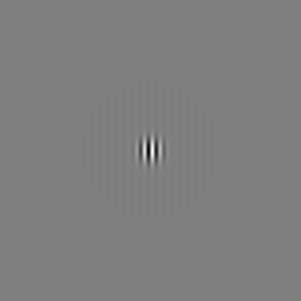
\includegraphics[scale=0.1]{ch4/figures/iGabor1_0.jpg}
 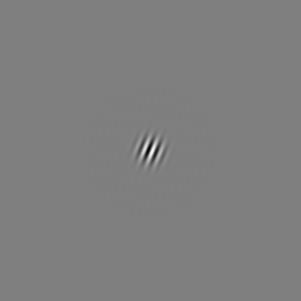
\includegraphics[scale=0.1]{ch4/figures/iGabor1_1.jpg}
 \includegraphics[scale=0.1]{ch4/figures/iGabor1_2.jpg}
 \includegraphics[scale=0.1]{ch4/figures/iGabor1_3.jpg}
 \includegraphics[scale=0.1]{ch4/figures/iGabor1_4.jpg}
 \includegraphics[scale=0.1]{ch4/figures/iGabor1_5.jpg}
 \includegraphics[scale=0.1]{ch4/figures/iGabor1_6.jpg}
 \includegraphics[scale=0.1]{ch4/figures/iGabor1_7.jpg}\\
 \includegraphics[scale=0.1]{ch4/figures/iGabor2_0.jpg}
 \includegraphics[scale=0.1]{ch4/figures/iGabor2_1.jpg}
 \includegraphics[scale=0.1]{ch4/figures/iGabor2_2.jpg}
 \includegraphics[scale=0.1]{ch4/figures/iGabor2_3.jpg}
 \includegraphics[scale=0.1]{ch4/figures/iGabor2_4.jpg}
 \includegraphics[scale=0.1]{ch4/figures/iGabor2_5.jpg}
 \includegraphics[scale=0.1]{ch4/figures/iGabor2_6.jpg}
 \includegraphics[scale=0.1]{ch4/figures/iGabor2_7.jpg}\\
 \includegraphics[scale=0.1]{ch4/figures/iGabor3_0.jpg}
 \includegraphics[scale=0.1]{ch4/figures/iGabor3_1.jpg}
 \includegraphics[scale=0.1]{ch4/figures/iGabor3_2.jpg}
 \includegraphics[scale=0.1]{ch4/figures/iGabor3_3.jpg}
 \includegraphics[scale=0.1]{ch4/figures/iGabor3_4.jpg}
 \includegraphics[scale=0.1]{ch4/figures/iGabor3_5.jpg}
 \includegraphics[scale=0.1]{ch4/figures/iGabor3_6.jpg}
 \includegraphics[scale=0.1]{ch4/figures/iGabor3_7.jpg}\\
 \includegraphics[scale=0.1]{ch4/figures/iGabor4_0.jpg}
 \includegraphics[scale=0.1]{ch4/figures/iGabor4_1.jpg}
 \includegraphics[scale=0.1]{ch4/figures/iGabor4_2.jpg}
 \includegraphics[scale=0.1]{ch4/figures/iGabor4_3.jpg}
 \includegraphics[scale=0.1]{ch4/figures/iGabor4_4.jpg}
 \includegraphics[scale=0.1]{ch4/figures/iGabor4_5.jpg}
 \includegraphics[scale=0.1]{ch4/figures/iGabor4_6.jpg}
 \includegraphics[scale=0.1]{ch4/figures/iGabor4_7.jpg}\\
\end{center}
\caption{The imaginary part of the $5\times8$ Gabor wavelets.}
\label{fig:imaggabor}
\end{figure} 

\subsubsection{Gabor Wavelet Transform}
In computer vision, feature stands for piece of ``interesting'' information which is relevant for solving a specific vision application, such as Face recognition. In appearance based approaches, features refer to the result after a general neighbourhood operation applied on an image. The result contains local or global information which contribute to resolve the specific vision problem. An image can be represented by a group of features.  Computer vision system will deal with the features rather than the image directly. 
The extraction of feature is  defined in terms of local neighbourhood operations. In the thesis, Gabor wavelet transform is defined as the approach to extract the features which are relevant to face recognition. Since the selective schemes available for frequency range and orientation interval, Gabor wavelets are ideal for extracting features on face images. 
\paragraph{Why Gabor is important for Face Recognition}
To be written \ldots


\paragraph{Convolution}
The Gabor wavelet transform is the course of two-dimensional convolution of an image with a family of Gabor wavelets kernels defined by \mbox{Equation}\ref{eq:kernel}.  Two-dimensional (2-D) convolution is a specific type of local neighbourhood operation which is belong to the linear approach to image analysis. The 2-D convolution $g$ of two-dimensional functions $f$ and $h$ is denoted by $f*h$. The function of 2-D convolution is described as
\newcommand{\ud}{\mathrm{d}}
{\setlength\arraycolsep{2pt}
\begin{eqnarray}\label{eq:conv2}
 g(x, y) = \int_{-\infty}^{\infty}\int_{-\infty}^{\infty}f(a,b)h(x-a,y-b) \, \ud a \, \ud b \nonumber\\
= \int_{-\infty}^{\infty}\int_{-\infty}^{\infty}f(x-a,y-b)h(a,b) \, \ud a \, \ud b \nonumber\\
= (f*h)(x,y) = (h*f)(x,y) 、
\end{eqnarray}
} 
where $*$ symbolise the convolution operator. The 2-D convolution is an integral of the functions $f$ and $h$. The convolution means a linear filtering process using the filter $h$ on the image $f$.  The linear filtering is often used in local image pre-processing.
\paragraph{2D discrete convolution}
In two-dimensional discrete image domain, the linear filtering calculate the resulting value in the image pixel $g(x,y)$ as a linear combination of the pixel value in a local neighbourhood of the pixel $f(a,b)$  The 2-D discrete convolution is described as
\begin{equation}
 %g(x,y)=\sum^{\infty}_{a=-\infty}\sum^{\infty}_{b=-\infty}f(a,b)h(x-a,y-b)
g(x,y)=\sum_{a}\sum_{b}f(a,b)h(x-a,y-b)
\end{equation}
where $f(a,b)$ is the 2-D discrete input image and $h(x,y)$ is so called \textbf{convolution mask} or convolution kernel.The convolution mask is often used with an odd number number of pixels in rows and columns, such as $3\times3$, $5\times5$ and so on. A example \cite{Davies1990} of $3\times3$ convolution mask is like
\begin{displaymath}
 \left[  \begin{array}{ccc}
          \mathrm{h}_{4} &\mathrm{h}_{3} & \mathrm{h}_{2} \\
	  \mathrm{h}_{5} & \mathrm{h}_{0} & \mathrm{h}_{1} \\
	  \mathrm{h}_{6} & \mathrm{h}_{7} & \mathrm{h}_{8} 
         \end{array}
\right ]
\end{displaymath}
where $\mathrm{h}_{n}$ is the coefficient of the convolution mask. The 2-D convolution result is the linear neighbourhood operation weighted by the corresponding coefficients in the mask $h$. In practice, fast convolution is used to increase the speed of the convolution. Fast convolution algorithm consists of taking the fast Fourier transform (FFT) of the input image and the convolution mask, multiplying them together, and then performing the inverse fast Fourier transform (IFFT). In the thesis, the 2-D discrete convolution function is provided by OpenCV\cite{}.
\paragraph{The Size of Mask}
The size of a Gabor filtering convolution mask is important. The size of a mask should not be small, otherwise the properties of frequency and orientation of Gabor will not be expressed, e.g. if the size of mask is small, only part of Gabor can be displayed. The size of a mask should not be large, otherwise more computation on convolution will be cost, and some computation is time-wasting. For an instance, in \mbox{Figure} \ref{fig:realgabor}, the size of the the Gabor convolution masks is $301\times301$, and the Gabors with the lowest frequency are shown in the top row. The span of these Gabor masks only possess very small part area of the whole mask. The rest area is flat which means zero or no information. The most area of the mask contains no information so that most of computation will be wasted if convolution applied.  Therefore, there is a trade-off between the integrality of a Gabor and computation effectiveness of convolution. The size of a Gabor mask need to cover the whole Gabor. Because Gabor is the product of a Gaussian function with a complex wave, the size of the Gabor mask need to cover the spatial extent of Gaussian. The extent of Gaussian is determined by the spatial frequency $\nu$ and the derivation of Gaussian function $\sigma$ in \mbox{Equation} \ref{eq:kernel}  According to Dunn et al\cite{Dunn1995}, the Gabor filter were truncated to six times of the span of Gaussian function. The span of Gaussian function is $\frac{\sigma}{\|k_{\nu}\|}$ and $k_{\nu}=\frac{k_{max}}{f^{\nu}}$, so that the Gabor mask is truncated to a width $W$
 \begin{equation}
  W  = \frac{6\sigma}{\|k_{\nu}\|}+1 = 6 f^{\nu}\frac{\sigma}{k_{max}}+1
 \end{equation}
In the thesis, the maximum frequency is $k_{max}=\frac{\pi}{2}$, the factor $f = \sqrt{2}$ and the standard derivation of the Gaussian $\sigma=2\pi$, so the width is 
\begin{equation}
 W = 24\cdot2^{\frac{\nu}{2}}+1
\end{equation}
Because $W$ should be an odd integer, for five different spatial frequencies $\nu\in\{-1,\ldots,3\}$, the corresponding sizes of Gabor filtering masks are $19\times19$, $25\times25$, $35\times35$, $49\times49$ and $69\times69$. \mbox{Figure} \ref{fig:fivemasks} shows when orientation is $\frac{3\pi}{8}$, the corresponding real masks with the different spatial frequencies.
\begin{figure}
\begin{center}
\includegraphics[scale=1.0]{ch4/figures/real-1.jpg}
\includegraphics[scale=1.0]{ch4/figures/real0.jpg}
\includegraphics[scale=1.0]{ch4/figures/real1.jpg}
\includegraphics[scale=1.0]{ch4/figures/real2.jpg}
\includegraphics[scale=1.0]{ch4/figures/real3.jpg}\\
\caption{When the orientation is $\frac{3\pi}{8}$, the corresponding Gabor filtering convolution masks with the five different spatial frequencies $\nu\in\{-1,\ldots,3\}$.} 
\end{center}
\label{fig:fivemasks}
\end{figure} 

\paragraph{Magnitude Response} 
To get Gabor wavelet transform of an image, the 40 Gabor wavelets are convolved with the image. Let $I(z)$, where $z=(x,y)$ define the position in the image, the convolution of image $I$ and a Gabor kernel $\psi_{\mu,\nu}$ is defined as follows
\begin{equation}\label{eq:conv}
 O_{\mu,\nu}(z)=I(z)\ast\psi_{\mu,\nu}(z)
\end{equation}
where $*$ denotes the convolution operator, and $O_{\mu,\nu}$ is the convolution result corresponding to the Gabor kernel at the orientation $/mu$ and the spatial frequency i.e. scale $\nu$.
Since Gabor wavelets is of the complex form, so that the convolution results contain the real response and imaginary response as follow
\begin{displaymath}
 O_{\mu,\nu}(z) = \Re\{O_{\mu,\nu}(z)\} +i\,\Im\{O_{\mu,\nu}(z)\}
\end{displaymath}
The real response of Gabor filtering is an image $I(z)$ convolved with the real unit of Gabor kernel described as (\ref{eq:real}). The real response of Gabor filtering is 
\begin{equation}
 \Re\{O_{\mu,\nu}(z)\} = I(z) *  \Re\{\psi_{\mu,\nu}\}
\end{equation}
The imaginary response is the image convolved with the imaginary unit described as (\ref{eq:imag}). The imaginary responses of Gabor filtering is 
\begin{equation}
 \Im\{O_{\mu,\nu}(z)\} = I(z) *  \Im\{\psi_{\mu,\nu}\}
\end{equation}
where $z = (x,y)$ define the position in an image which contains the grey level distribution. Given a face image showed in \mbox{Figure} \ref{fig:afaceimage} in the \textbf{FERET} database, the 40 Gabor real responses are displayed in \mbox{Figure} \ref{fig:realresponses}; the 40 Gabor imaginary responses are displayed in \mbox{Figure} \ref{fig:imagresponses}.
\begin{figure}
 \begin{center}
   \includegraphics[scale=0.75]{ch4/figures/FERET.jpg}
   \caption{A face image selected from the \textbf{FERET} database}
   \label{fig:afaceimage}
 \end{center}
\end{figure} 

\begin{figure}
 \begin{center}
  \includegraphics[scale=0.5]{ch4/figures/real_-1_0.jpg}
  \includegraphics[scale=0.5]{ch4/figures/real_-1_1.jpg}
  \includegraphics[scale=0.5]{ch4/figures/real_-1_2.jpg}
  \includegraphics[scale=0.5]{ch4/figures/real_-1_3.jpg}
  \includegraphics[scale=0.5]{ch4/figures/real_-1_4.jpg}
  \includegraphics[scale=0.5]{ch4/figures/real_-1_5.jpg}
  \includegraphics[scale=0.5]{ch4/figures/real_-1_6.jpg}
  \includegraphics[scale=0.5]{ch4/figures/real_-1_7.jpg}\\
  \includegraphics[scale=0.5]{ch4/figures/real_0_0.jpg}
  \includegraphics[scale=0.5]{ch4/figures/real_0_1.jpg}
  \includegraphics[scale=0.5]{ch4/figures/real_0_2.jpg}
  \includegraphics[scale=0.5]{ch4/figures/real_0_3.jpg}
  \includegraphics[scale=0.5]{ch4/figures/real_0_4.jpg}
  \includegraphics[scale=0.5]{ch4/figures/real_0_5.jpg}
  \includegraphics[scale=0.5]{ch4/figures/real_0_6.jpg}
  \includegraphics[scale=0.5]{ch4/figures/real_0_7.jpg}\\
  \includegraphics[scale=0.5]{ch4/figures/real_1_0.jpg}
  \includegraphics[scale=0.5]{ch4/figures/real_1_1.jpg}
  \includegraphics[scale=0.5]{ch4/figures/real_1_2.jpg}
  \includegraphics[scale=0.5]{ch4/figures/real_1_3.jpg}
  \includegraphics[scale=0.5]{ch4/figures/real_1_4.jpg}
  \includegraphics[scale=0.5]{ch4/figures/real_1_5.jpg}
  \includegraphics[scale=0.5]{ch4/figures/real_1_6.jpg}
  \includegraphics[scale=0.5]{ch4/figures/real_1_7.jpg}\\
  \includegraphics[scale=0.5]{ch4/figures/real_2_0.jpg}
  \includegraphics[scale=0.5]{ch4/figures/real_2_1.jpg}
  \includegraphics[scale=0.5]{ch4/figures/real_2_2.jpg}
  \includegraphics[scale=0.5]{ch4/figures/real_2_3.jpg}
  \includegraphics[scale=0.5]{ch4/figures/real_2_4.jpg}
  \includegraphics[scale=0.5]{ch4/figures/real_2_5.jpg}
  \includegraphics[scale=0.5]{ch4/figures/real_2_6.jpg}
  \includegraphics[scale=0.5]{ch4/figures/real_2_7.jpg}\\
  \includegraphics[scale=0.5]{ch4/figures/real_3_0.jpg}
  \includegraphics[scale=0.5]{ch4/figures/real_3_1.jpg}
  \includegraphics[scale=0.5]{ch4/figures/real_3_2.jpg}
  \includegraphics[scale=0.5]{ch4/figures/real_3_3.jpg}
  \includegraphics[scale=0.5]{ch4/figures/real_3_4.jpg}
  \includegraphics[scale=0.5]{ch4/figures/real_3_5.jpg}
  \includegraphics[scale=0.5]{ch4/figures/real_3_6.jpg}
  \includegraphics[scale=0.5]{ch4/figures/real_3_7.jpg}
 \end{center}
\caption{The 40 real response images. The face image shown in \mbox{Figure} \ref{fig:afaceimage} is convolved with the real unit of these 40 Gabor wavelets.}
\label{fig:realresponses}
\end{figure} 

\begin{figure}
 \begin{center}
  \includegraphics[scale=0.5]{ch4/figures/imag_-1_0.jpg}
  \includegraphics[scale=0.5]{ch4/figures/imag_-1_1.jpg}
  \includegraphics[scale=0.5]{ch4/figures/imag_-1_2.jpg}
  \includegraphics[scale=0.5]{ch4/figures/imag_-1_3.jpg}
  \includegraphics[scale=0.5]{ch4/figures/imag_-1_4.jpg}
  \includegraphics[scale=0.5]{ch4/figures/imag_-1_5.jpg}
  \includegraphics[scale=0.5]{ch4/figures/imag_-1_6.jpg}
  \includegraphics[scale=0.5]{ch4/figures/imag_-1_7.jpg}\\
  \includegraphics[scale=0.5]{ch4/figures/imag_0_0.jpg}
  \includegraphics[scale=0.5]{ch4/figures/imag_0_1.jpg}
  \includegraphics[scale=0.5]{ch4/figures/imag_0_2.jpg}
  \includegraphics[scale=0.5]{ch4/figures/imag_0_3.jpg}
  \includegraphics[scale=0.5]{ch4/figures/imag_0_4.jpg}
  \includegraphics[scale=0.5]{ch4/figures/imag_0_5.jpg}
  \includegraphics[scale=0.5]{ch4/figures/imag_0_6.jpg}
  \includegraphics[scale=0.5]{ch4/figures/imag_0_7.jpg}\\
  \includegraphics[scale=0.5]{ch4/figures/imag_1_0.jpg}
  \includegraphics[scale=0.5]{ch4/figures/imag_1_1.jpg}
  \includegraphics[scale=0.5]{ch4/figures/imag_1_2.jpg}
  \includegraphics[scale=0.5]{ch4/figures/imag_1_3.jpg}
  \includegraphics[scale=0.5]{ch4/figures/imag_1_4.jpg}
  \includegraphics[scale=0.5]{ch4/figures/imag_1_5.jpg}
  \includegraphics[scale=0.5]{ch4/figures/imag_1_6.jpg}
  \includegraphics[scale=0.5]{ch4/figures/imag_1_7.jpg}\\
  \includegraphics[scale=0.5]{ch4/figures/imag_2_0.jpg}
  \includegraphics[scale=0.5]{ch4/figures/imag_2_1.jpg}
  \includegraphics[scale=0.5]{ch4/figures/imag_2_2.jpg}
  \includegraphics[scale=0.5]{ch4/figures/imag_2_3.jpg}
  \includegraphics[scale=0.5]{ch4/figures/imag_2_4.jpg}
  \includegraphics[scale=0.5]{ch4/figures/imag_2_5.jpg}
  \includegraphics[scale=0.5]{ch4/figures/imag_2_6.jpg}
  \includegraphics[scale=0.5]{ch4/figures/imag_2_7.jpg}\\
  \includegraphics[scale=0.5]{ch4/figures/imag_3_0.jpg}
  \includegraphics[scale=0.5]{ch4/figures/imag_3_1.jpg}
  \includegraphics[scale=0.5]{ch4/figures/imag_3_2.jpg}
  \includegraphics[scale=0.5]{ch4/figures/imag_3_3.jpg}
  \includegraphics[scale=0.5]{ch4/figures/imag_3_4.jpg}
  \includegraphics[scale=0.5]{ch4/figures/imag_3_5.jpg}
  \includegraphics[scale=0.5]{ch4/figures/imag_3_6.jpg}
  \includegraphics[scale=0.5]{ch4/figures/imag_3_7.jpg}
 \end{center}
\caption{The 40 imaginary responses}
\label{fig:imagresponses}
\end{figure} 

From \mbox{Figure} \ref{fig:realresponses} and \ref{fig:imagresponses}, there are some stripes cross the images, which shows no visual knowledge of individual and human face. Therefore, neither the real nor the imaginary response contributes to face detection or face recognition. 

Texture detection can be operated based on the magnitude of the output of the Gabor filtering \cite{Bovik1990}. The magnitude response of Gabor filtering is large to enable detection. Human face contains various texture, therefore the magnitude response of Gabor filtering will enhance the recognition on face. The magnitude response is the square root of the sum of squared real responses and imaginary responses, such as
\begin{equation}
 \|O_{\mu,\nu}(z)\| = \sqrt{\Re^2\{O_{\mu,\nu}(z)\} + \Im^2\{O_{\mu,\nu}(z)\}}
\end{equation}
It can be seen that the magnitude response is modulus. Same as the real and imaginary response, given the face image displayed in \mbox{Figure} ~\ref{fig:afaceimage}, the 40 Gabor magnitude responses are shown in \mbox{Figure} \ref{fig:magresponses}. The magnitude responses demonstrate local variance within low spatial-frequencies and global variance within high spatial-frequencies.  In the top rows, more precisive dissimilarity across the face are shown, while in the bottom rows, more high-level scale dissimilarity across the face are shown. In the thesis, the magnitude response of Gabor filtering is adopted to extract Gabor Wavelet Features. 
\begin{figure}
\begin{center}
 \includegraphics[scale=0.5]{ch4/figures/mag_-1_0.jpg}
 \includegraphics[scale=0.5]{ch4/figures/mag_-1_1.jpg}
 \includegraphics[scale=0.5]{ch4/figures/mag_-1_2.jpg}
 \includegraphics[scale=0.5]{ch4/figures/mag_-1_3.jpg}
 \includegraphics[scale=0.5]{ch4/figures/mag_-1_4.jpg}
 \includegraphics[scale=0.5]{ch4/figures/mag_-1_5.jpg}
 \includegraphics[scale=0.5]{ch4/figures/mag_-1_6.jpg}
 \includegraphics[scale=0.5]{ch4/figures/mag_-1_7.jpg}\\
 \includegraphics[scale=0.5]{ch4/figures/mag_0_0.jpg}
 \includegraphics[scale=0.5]{ch4/figures/mag_0_1.jpg}
 \includegraphics[scale=0.5]{ch4/figures/mag_0_2.jpg}
 \includegraphics[scale=0.5]{ch4/figures/mag_0_3.jpg}
 \includegraphics[scale=0.5]{ch4/figures/mag_0_4.jpg}
 \includegraphics[scale=0.5]{ch4/figures/mag_0_5.jpg}
 \includegraphics[scale=0.5]{ch4/figures/mag_0_6.jpg}
 \includegraphics[scale=0.5]{ch4/figures/mag_0_7.jpg}\\
 \includegraphics[scale=0.5]{ch4/figures/mag_1_0.jpg}
 \includegraphics[scale=0.5]{ch4/figures/mag_1_1.jpg}
 \includegraphics[scale=0.5]{ch4/figures/mag_1_2.jpg}
 \includegraphics[scale=0.5]{ch4/figures/mag_1_3.jpg}
 \includegraphics[scale=0.5]{ch4/figures/mag_1_4.jpg}
 \includegraphics[scale=0.5]{ch4/figures/mag_1_5.jpg}
 \includegraphics[scale=0.5]{ch4/figures/mag_1_6.jpg}
 \includegraphics[scale=0.5]{ch4/figures/mag_1_7.jpg}\\
 \includegraphics[scale=0.5]{ch4/figures/mag_2_0.jpg}
 \includegraphics[scale=0.5]{ch4/figures/mag_2_1.jpg}
 \includegraphics[scale=0.5]{ch4/figures/mag_2_2.jpg}
 \includegraphics[scale=0.5]{ch4/figures/mag_2_3.jpg}
 \includegraphics[scale=0.5]{ch4/figures/mag_2_4.jpg}
 \includegraphics[scale=0.5]{ch4/figures/mag_2_5.jpg}
 \includegraphics[scale=0.5]{ch4/figures/mag_2_6.jpg}
 \includegraphics[scale=0.5]{ch4/figures/mag_2_7.jpg}\\
 \includegraphics[scale=0.5]{ch4/figures/mag_3_0.jpg}
 \includegraphics[scale=0.5]{ch4/figures/mag_3_1.jpg}
 \includegraphics[scale=0.5]{ch4/figures/mag_3_2.jpg}
 \includegraphics[scale=0.5]{ch4/figures/mag_3_3.jpg}
 \includegraphics[scale=0.5]{ch4/figures/mag_3_4.jpg}
 \includegraphics[scale=0.5]{ch4/figures/mag_3_5.jpg}
 \includegraphics[scale=0.5]{ch4/figures/mag_3_6.jpg}
 \includegraphics[scale=0.5]{ch4/figures/mag_3_7.jpg}
 \caption{}
\end{center}
\label{fig:magresponses}
\end{figure} 

\subsubsection{Gabor Wavelet Feature}
\label{sec:gaborwaveletfeature}
A Gabor wavelet feature $j$ is configured by three key parameters: the position $z = (x,y)$, the orientation $\nu$, and the spatial frequency $\mu$. The value of a Gabor wavelet feature is the corresponding magnitude response of Gabor wavelet transform as illustrated as
\begin{equation}\label{eq:gaborfeature}
 j(z,\nu,\mu) =  \|O_{\mu,\nu}(z)\|
\end{equation}
The Gabor wavelet features vary in  the orientations, the frequencies and the positions. There are eight different orientations from $0$ to $\frac{7\pi}{8}$ with the interval $\frac{\pi}{8}$, and five different scales from $-1$ to $3$.  These 40 Gabor wavelets will be applied on every position on the face image, so that the total number of Gabor wavelet features is determined by the number of orientations, the number of scales, and the resolution (size) of the image  applied. For example, there is an image with $64\time64$ pixels, and the total number of Gabor wavelet features is $64\time64\time5\time8=163,840$. Because the number of Gabor wavelets is fixed, the only factor which change the total number of features is the size of the images. Also, on each pixel, there are 40 Gabor wavelet features available.  In general, to describe a Gabor wavelet feature, there are three factors: the position $z=(x,y)$, the orientation $\mu$, and the scale $\nu$.  The value of a Gabor wavelet feature obtained on an image is the magnitude response of the corresponding Gabor wavelet transform.


\subsection{AdaBoost}
\label{sec:faceveri:adaboost}
\subsubsection{Basic Idea}
AdaBoost, stand for Adaptive Boosting, is a machine learning algorithm, formulated by Freund and Schapire \cite{Freund1995,Freund1999,Schapire1999}. It can be usefully considered to have other significant algorithms on Pattern recognition. The AdaBoost can be used in conjunction with many other learning algorithms to improve their performance.  The Adaboost is to improve the accuracy of any learning algorithm.
\paragraph{Background}
Boosting is a general method which used to ``boost'' the accuracy of any given learning algorithm. Boosting is originated in a theoretical framework for machine learning called ``PAC'' (Probably Approximately Correct) learning model\cite{Valiant1984}. After the PAC releasing,  there is a discussion whether a ``weak'' learning algorithm performing just slightly better than random guessing can be ``boosted'' into an arbitrarily accurate ``strong'' learning algorithm. Kearns and Valiant \cite{Kearns1994} were first to response to the discussion. In 1989, Schapire proposed the first provable polynomial-time boosting algorithm. Boosting were first applied to a real-world OCR task, relying on neural networks as base learners in \cite{Drucker1993}. The AdaBoost is generally considered as a first step to more practical Boosting algorithm. Although  Freund and Schapire \cite{Freund1995,Freund1999,Schapire1999} claims that AdaBoost often tends not to overfit when running for a large number of iterations. However, simulations by \cite{Grove1998} on data sets with higher noise content could clearly show overfitting side-effects. Due to the accuracy of Boosting, the algorithm has been extend for regression \cite{Friedman1998}, multi-class classification \cite{Zhu2006}, and unsupervised learning \cite{Ratsch2002}. Recently, Boosting has been successfully implemented in various applications. OCR \cite{Drucker1993} is implemented, which used boosted classifier of neural network. In Human face detection \cite{Viola2001}, AdaBoost was used to train a ``string'' classifier to detect human faces in an image.
\paragraph{Horse-racing analogy}
The authors of AdaBoost draw an analogy between the AdaBoost algorithm and horse-racing gambling\cite{Freund1995,Freund1999,Schapire1999}. The gambling is that a horse-racing gambler whose purpose is to maximise his winning want to create a computer program helping him betting. The program will accurately predict the winner of a horse race based on usual information such as number of races recently won by each horse, betting odds for each horse, etc. To create such a program, he consults a successful horse-racing gambling expert for the optimal policy to bet. However, the expert failed to answer the optimal policy. because the expert can not articulate a grand set of rules for choosing a winning horse. On the other hand, when he presents the specific data of races, the expert can easily come up with a ``rule of thumb'' for the set of races. The possible ``rule of thumb'' is ``betting on the horse that has recently won the most races'' or ``betting on the horse with the most favoured odds''. The rule of thumb is very rough and moderately inaccurate, but the rule is still reasonable. The rule can be easily concluded from the specific data rather than from a random guess. If the gambler keeps on asking the expert on different collections of races, the expert will draw many rules of thumb. To get the maximum advantage from these rules of thumb, two problem must be resolved. They are
\begin{itemize}
 \item How could the gambler choose the collections of races which are given to the expert for extracting the most useful rules of thumb?
 \item  When many rules of thumb are extracted, how these rules combined into one single accurate rule?
\end{itemize}

\paragraph{AdaBoost}
AdaBoost is an efficient method of producing a highly accurate predication rule by combining a set of rough and moderately inaccurate rules of thumb..To computer vision and pattern recognition, the word ``rule'' is replaced by the word ``classifier'', ``learner'', ``hypothesis'', etc. In the thesis, due to face recognition, the term ``classifier'' will be used.  In general, the so-called ``rule of thumb'' is simply designed rules which give low accuracy over long-term oberservation. For the term``rule of thumb'', it will be called ``weak learner'' or ``weak classifier'', because it comes up with low accuracy. AdaBoost refers to a method of combining a set of ``weak'' classifiers into an ``strong'' classifier which gives a high prediction accuracy. In order to design the ``strong'' classifier, there are two issues need to resolved
\begin{itemize}
 \item How is a set of ``weak'' classifiers organised into a ``strong'' classifier?
 \item How is a ``weak'' classifier is selected so that it is contributed to a ``strong'' classifier?
\end{itemize}
AdaBoost resolves these two problems and gives the best performacne of classification.

The AdaBoost algorithm is introduced to solve the difficulties of the earlier boosting algorithm. Boosting is rooted in a machine learning framework called the ``PAC'' learning model. The idea of the PAC model is that a ``weak'' classifier which performs slightly better than random guessing. The PAC model can be ``boosted'' into a ``strong'' classifier. AdaBoost is an \textit{adaptive} Boosting algorithm, because AdaBoost adapts to the error rates of individual ``weak'' classifier. Pseudocode for AdaBoost is given in \mbox{Table} \ref{tab:adaboost}. 

\paragraph{Training Data}There are $n$ examples in the training set $(x_{1},y_{1}),\ldots,(x_{n},y_{n})$. $x$ is the data of the example which can be integer or real, positive or negative. $y$ is the label of the example. It is assumed that $y \in {0,1}$ i.e. $y = 0$ or $y = 1$. There are two labels so that the algorithm is dealing with the two-class classification problem. In this section, only the two-class classification is discussed. AdaBoost maintains a collection of weights on each example. All the weights $\omega_{t}$ are kept as a probability distribution $D_{t}$.
\begin{equation}\label{eq:distribution}
 D_{t}(i) = \omega_{t,i}
\end{equation}
At the beginning, the distribution $D_{t}$ is uniform that all weights are equal to $1/n$. 

\paragraph{Weak Learner}
AdaBoost processes ``weak'' classifier repeatedly in $t=1,\ldots,T$ iteration. During each iteration, a ``weak'' learner $h_{t}$ is trained by using the distribution $D_{t}$. To train a weak learner, there are many approaches to do the task, e.g. Naive Bayes\cite{Domingos1997}, Perceptron\cite{Rosenblatt1958}, Linear discriminant analysis (LDA)\cite{Martinez2001}, Neural network\cite{Riedmiller1993}, etc. After $h_{t}$ is trained, calculation of the error $\varepsilon_{t}$ of the weak learner is described in \mbox{Equation} \ref{eq:error}.. When an example $(x_{i},y_{i})$ is mis classified by the weak learner $h_{t}$, i.e. $h_{t}(x_{i})\neq y_{i}$, the weight  $\omega_{t,i}$ will be counted in the error $\varepsilon_{t}$. When an example is classified, the weight will not be counted in $\varepsilon_{t}$. The goodness of a weak learner is measured by its error $\varepsilon_{t}$. If $\varepsilon_{t}$.becomes small, the classification ability of the weak learner becomes ``stronger''. Because the basic idea of AdaBoost is to combine some weak rules into a strong one, to the weak learner, the error $\varepsilon_{t}$ is not required to relay in very small number range. Normally, the error $\varepsilon_{t}$ is relative large, but not exceed 0.5. In practice, the weak learner may be an algorithm that can use the weights $\omega_{t,i}$ on the training data. Alternatively, when the weights can not be applied on training procedure, a subset of the training data can be sampled according to the distribution $D_{t}$, and those unweighted resampled data can be used to train the weak learner. Recalling the horse-racing analogy, in the example $(x_{i},y_{i})$, $x_{i}$ correspond to information revelant to horse races, e.g. the name of horse, the odds, the track record of horse, the weather of the racing day, the condition of race course, etc.  The label $y_{i}$ gives the result of each race, i.e. who is the winner. The weak learners are the rules of thumb given by the expert. 

\paragraph{Importance}Once the weak learner has been trained, AdaBoost will determin a parameter $\alpha_{t}$. The parameter $\alpha_{t}$ indicates how important the corresponding weak learner $h_{t}$ is  in the final classifier $H(x)$. When $\alpha_{t}$ is bigger, corresponding weak learner $h_{t}$ contributes greater in $H(x)$  Note that $alpha_{t} \geq 0$ if $\varepsilon_{t} \leq \frac{1}{2}$, and that $\alpha_{t}$ gets larger as $\varepsilon_{t}$ gets smaller.

\paragraph{Updating}The weight $\omega_{t,i}$ is updated using the rule shown in \mbox{Equation} \ref{eq:update}. When weak learner $h_{t}$ classifies the example $x_{i}$ correctly, the weight is multiplied by $e^{-\alpha_{t}}$ which lead decrease in the weight. When $h_{t}$ mis-classifies the example  $x_{i}$, the weight is multiplied by $e^{\alpha_{t}}$, which lead increase in the weight. The effect of the updating weight is to increase the weight of examples misclassified, and to decrease the weight of correctly classified examples. In this way, AdaBoost is modulated to focus on those examples which are ``hard'' to be classified.

\paragraph{Normalisation}The updated weights are normalised by a normalisation operator $Z_{t}$. After updating the weights, all the weights may not constitute a probability distribution, i.e. the sum of all weights may not be equal to $1$. To forge the weights into a probability distribution, all the weight for the next iteration will be normalised according to \mbox{Equation} \ref{eq:normalisation}.  Hence, from $t$ round to $t+1$ round, it is not certian that the weight $\omega_{t+1,i}$ must be increased over  $\omega_{t,i}$ if misclassified, or the weight  $\omega_{t+1,i}$ must be decreased over  $\omega_{t,i}$ if classified correctly. However,  $\omega_{t+1,i}$ is increased to the example $x_{i}$ over other examples, when $x_{i}$ is misclassified and other examples are classified correctly in the $t$th round. In general, the weights are only increase or decrease relatively, but not absolutely.

\paragraph{Final classifier}
The final ``strong'' classifier $H(x)$ is a weighted majority vote of the $T$ weak learners where $\alpha_{t}$ is the weight assigned to $h_{t}$.

\begin{table}
$AdaBoost$
\begin{algorithmic}[1]
\STATE Given the training set $(x_{1},y_{1}),\ldots,(x_{n},y_{n})$, where $x_{i}$ is the data of the $i$th example, and $y_{i} \in Y=\{0,1\}$.
\STATE Initialise the weights $\omega_{1,i}=\frac{1}{n}$ for each example $(x_{i},y_{i})$.
\FOR{$t=1,\ldots,T$}
	\STATE Train a weak learner $h_{t}$ using the weights $\omega_{t,i}$.
	\STATE Get the weak learner with error 
                       \begin{equation}\label{eq:error}
                        \varepsilon_{t} =\sum_{i=0}^{n}\omega_{t,i}\|h_{t}(x_{i})-y_{i}\|^2
                       \end{equation}
	\STATE Choose $\alpha_{t}=\frac{1}{2}\ln \left( \frac{1-\varepsilon_{t}}{\varepsilon_{t}} \right)$
	\STATE Update the weights 
		\begin{equation}\label{eq:update}
		 \omega_{t,i} = \omega_{t,i} \times
                 \left\{
		  \begin{array}{ll}
		                                            e^{-\alpha_{t}} & \textrm{if $h_{t}(x_{i})=y_{i}$} \\
						           e^{\alpha_{t}} & \textrm{if $h_{t}(x_{i}) \neq y_{i}$}
		  \end{array}
		\right.
		\end{equation}
	\STATE Normalise the weights 
		\begin{equation}\label{eq:normalisation}
		  \omega_{t+1,i} = \frac{\omega_{t,i}}{\sum_{i=1}^{n}\omega_{t,i}}
		\end{equation}
	where the normalisation can be expressed by a normalisation factor $Z_{t}$ so that all $ \omega_{t+1,i}$ will keep a probability distribution.
\ENDFOR
\STATE The final ``strong'' classifier:
	\begin{equation}
	 H(x)  = 
		\left\{
		 \begin{array}{ll}
		  1 & \sum_{t=1}^{T}\alpha_{t}h_{t}(x) \geq \frac{1}{2}\sum_{t=1}^{T}\alpha_{t}\\
			\\
		  0 & \textrm{otherwise}
		 \end{array}
		\right. 
	\end{equation}
\end{algorithmic}
\caption{The AdaBoost algorithm}
\label{tab:adaboost}
\end{table} 

\paragraph{Training error}
AdaBoost is concerned to reduce the training error in the most basic theoretical properties. The error $\varepsilon_{t}$ of $h_{t}$ can be replaced by $(\frac{1}{2}-\gamma_{t})$. $\gamma_{t})$ measures how much $h_{t}$ is better than random guessing. The training error of the final classifier $H$ is at most
\begin{equation} \label{eq:trainingerror}
 \prod_{t}[2\sqrt{\varepsilon_{t}(1- \varepsilon_{t})}] = \prod_{t}\sqrt{1-4\gamma_{t}^{2}}  \leq e^{-2\sum_{t}\gamma_{t}^{2}}
\end{equation}
From \mbox{Equation} \ref{eq:trainingerror}, if each weak learner is slightly better than random guessing, i.e. $\gamma_{t}>\gamma$ for some $0<\gamma<\frac{1}{2}$, then the training error drops exponentially fast.

\subsubsection{Constructing a strong classifier}
In \cite{}, it gives a landscape how a strong classifier is constructed. \mbox{Figure} \ref{fig:howtostrongclassifier} displays that how some weak learners can be constructed into a final strong classifier. The original training data is shown in the top-left of \mbox{Figure} \ref{fig:howtostrongclassifier}. There are many points which represent the training examples: blue examples are labelled as the positive data and red examples are labelled the negative data. The positive examples mold as a random Gaussian distribution $N(0,1)$ with centered at the origin $0$ and standard deviation $1$. Outside of the positive examples, the negative examples encircle the positive examples, which foumaleted as $\frac{1}{r\sqrt{8\pi^{3}}}e^{-1/2(r-4)^{2}}$ with $r$ indicating the radius of the negative data. The original training data is not linear separated, but non-linear separated. By using linear classification techniques, it is very difficult to discriminate the positive and negative examples. When the training data and initial weighting are ready, AdaBoost is started into the first iteration $t=1$.  In $t=1$, the algorithm is to find a weak learner $h_{1}$. Because there are many possible solution for weak learner, an optimal weak learner is found by minimizing the weighted training error $\varepsilon_{1}$. Due to adapt perceptron as weak learner, the weak learner $h_{1}$ is exhibited as a line in the top-right of \mbox{Figure} \ref{fig:howtostrongclassifier}  The line separates the training examples into two categories: plausible positive and plausible negative. According to perceptron, the examples above the line are considered as plausible negative, and the examples below the line are considered as plausible positive. As the left of the second row in \mbox{Figure} \ref{fig:howtostrongclassifier}, the examples are classified by the first weak learner, the green area reflects the plausible negative, and the yellow area reflects the plausible positive examples. After the weak learner $h_{1}$ is decided, the weights $\omega_{1}$ are updated with respect to the importance $\alpha_{1}$. In the iteration $t=2$, the weak learner $h_{2}$ is shown in the right of the second rows of the \mbox{Figure}. Because the importance $\alpha_{2}$ on the iteration is not significant, the classification result still keeps same as the first iteration, i.e. the plausible postive and the plausible negative area still keep same. Also from \mbox{Figure} \ref{fig:errorconverge}, it shows that the classification error on the first and the second iteration are same. When the algorithm comes to the third iteration, the third weak learner $h_{3}$ is found and displayed in the left of the third row in \mbox{Figure} \ref{fig:howtostrongclassifier}. The weak learner $h_{4}$ outlines the right-bottom boundary of the negative examples. The positive examples are constrained between the weak learner $h_{1}$ and $h_{2}$. The plausible positve area covers most positive examples, and the plausible negative area covers most negative examples, so that the classification error in \mbox{Figure} \ref{fig:errorconverge} is drop very significant in the iteration $t=3$. When AdaBoost comes into the iteration $t=4$ as shown in the right of the third row in \mbox{Figure} \ref{fig:howtostrongclassifier}, the fourth weak learner is found. The weak learner $h_{4}$ defines the left boundary of the negative examples, so that many negative examples are misclassified as the positive examples. In \mbox{Figure} \ref{fig:errorconverge}, the classification error grows very quickly. When the algorithm comes into the iteration $t=5$ as shown in the left of the fourth row in \mbox{Figure} \ref{fig:howtostrongclassifier}, the positive examples are constrained in a triangle area, and the classification error drops again. When AdaBoost goes to the iteration  $t=6$ and $t=7$, the positive examples are more restricted in a smaller area constructed by weak learners and the classification error continues to drop. Finally, AdaBoost goes into the iteration $t=40$, the positive examples are outlined by many weak learners, and the classification error converge to 0.05. 

From \mbox{Figure} \ref{fig:howtostrongclassifier}, it is seen that AdaBoost can be considered to use many weak learners to fit the training data. The weak learners outline the boundary of the positive examples. 
\begin{figure}
\begin{center}
 \includegraphics[angle=270, scale=0.166]{ch4/figures/56.pdf}
 \includegraphics[angle=270, scale=0.166]{ch4/figures/60.pdf}\\
 \includegraphics[angle=270, scale=0.166]{ch4/figures/59.pdf}
 \includegraphics[angle=270, scale=0.166]{ch4/figures/79.pdf}\\
 \includegraphics[angle=270, scale=0.166]{ch4/figures/81.pdf}
 \includegraphics[angle=270, scale=0.166]{ch4/figures/83.pdf}\\
 \includegraphics[angle=270, scale=0.166]{ch4/figures/85.pdf}
 \includegraphics[angle=270, scale=0.166]{ch4/figures/87.pdf}\\
 \includegraphics[angle=270, scale=0.166]{ch4/figures/89.pdf}
 \includegraphics[angle=270, scale=0.166]{ch4/figures/91.pdf}\\
\end{center}
\caption{The summary of AdaBoost}
\label{fig:howtostrongclassifier}
\end{figure} 

\begin{figure}
 \begin{center}
  \includegraphics[scale=0.33]{ch4/figures/92.pdf}
 \end{center}
\caption{Classification error converge}
\label{fig:errorconverge}
\end{figure} 

\subsubsection{Weak Learner}
The goal of AdaBoost is to find a final strong classifier with low error relative to thw weights $\omega_{t}$ over the training examples.On iteration $t$, a distribution $D_{t}$ is computed by normalising these weights. This distribution is fed to the weak learner which has small error with respect to the distribution. The weak learner deals with the training examples and the distribution, rather than the training examples themselves. In practice, there are two ways to process the examples and the weights.
\begin{itemize}
 \item The weak learner may be an algorithm that can use the distribution $D_{t}$ on the training examples.
 \item The training examples can be sampled according the distribution $D_{t}$, and these (unweighted) resampled examples can be used to train the weak learner.
\end{itemize}
The most straightforward way to train a weak learner with the training examples with respect to the weight is RPROP\cite{Riedmiller1993} Aritifical Neural Network algorithm. In OpenCV, RPROP algorithm has been implemented as a class with an interface for inputting examples and corresponding weights. The alternative way is to adapt a Naive Bayes classifier as the weak learner, and resample the examples according to the weights.
\paragraph{Weak Learner: ANN:RPROP}
An artificial neural network (ANN) is a mathematical model or computational model based on biological neural networks. It contains an interconnected group of artificial neurons. These are essentially simple mathematical models defining a function $f : X \rightarrow Y$. Each type of ANN model corresponds to a class of such functions.\\
In the thesis, OpenCV Machine Learning (ML) library was adapted. ML implements feedforward ANN. More particularly the ANN is multi-layer perceptrons (MLP), which is the most commonly used type of neural networks. MLP consists of the input layer, output layer and one or more hidden layers. Each layer of MLP contains one or more neurons that are directionally linked with the neurons from the previous and the next layer. \\
All the neurons in MLP are similar. Each neuron has several input, i.e. it takes the output values from several neurons in the previous layer on input. Each neuron has several output, i.e. it passes the response to several neurons in the next layer. The values computed from the previous layer are summed with certain weights, individual for each neuron, plus a bias term, and the sum is transformed using an activation function. \\
The larger the network size (the number of hidden layers and their sizes), the more is the potential network flexibility, and the error on the training set could be made arbitrarily small. But at the same time the learned network will also "learn" the noise present in the training set, so the error on the test set usually starts increasing after the network size reaches some limit. Besides, the larger networks are train much longer than the smaller ones. To build a ANN weak learner, it is not neccessary to design a large network, but a simple network. For an ANN:RPROP weak learner, input layer includes the number of neurons equal to the number of elements in the examples, e.g. if each example contains $m$ digits (i.e. a $m$ length vector), in the input layer, it should has $m$ neurons. There is one hidden layer including two neurons. Output layer includes one neuron which gives positive or negative results. \mbox{Figure} \ref{fig:annstructure} shows the ANN structure in the thesis.\\
One of the main problems with MLPs, when the number of selected features increases, is to find a good topology for the network, is to train the network,  and is to learn the training examples without overfitting.  A practical way to acquire MLP with good generalisation is to use weight decay regularization in learning. The purpose of the weight decay is to exclude the overfitting of the training set and hence to improve generalisation. Many different types of nonlinear optimisation methods exist for MLP training. In regularization, the RPROP (Resilient backpropagation) \cite{Riedmiller1993} algorithm has shown to perform well, and we also selected this method to be combined with the weight decay.\\
ML library in OpenCV implements a batch RPROP algorithm for training MLPs.  The training function of ANN is defined as
\begin{figure}
\begin{center}
  \includegraphics{ch4/figures/annstructure.png}
\end{center}
\caption{}
\label{fig:annstructure}
\end{figure}
\lstset{language=C++}
\lstset{basicstyle=\scriptsize\ttfamily,
showspaces=false,
showtabs=false,
columns=fixed,
frame=none,
%numbers=left,
numberstyle=\scriptsize,
breaklines=true,
showstringspaces=false,
xleftmargin=1cm
}
\begin{lstlisting}
int CvANN_MLP::train( const CvMat* _inputs, const CvMat* _outputs, const CvMat* _sample_weights, const CvMat* _sample_idx=0, CvANN_MLP_TrainParams _params = CvANN_MLP_TrainParams(), int flags=0 );
\end{lstlisting}

\_input is a floating-point matrix of input examples, one example per row. {\_output} is a floating-point matrix of the corresponding output, one output of example per row. 
 sample\_weights is only valid when using RPROP. It is an optional floating-point vector of weights for each example. Some examples may be more important than others for the training. The weights $ \omega_{t,i} $ are feed to the ANN weak learner by using this parameter. 
{\_sample\_idx} is the optional integer vector indicating the examples  that are taken into account. 
{\_params} is a structure for training parameters. 
{\_flags} are the various parameters to control the training algorithm.
\paragraph{Weak Learner: Naive Bayes}
A naive Bayes classifier is a simple probabilistic classifier based on applying Bayes' theorem with strong independence assumptions. Depending on the precise nature of the probability model, naive Bayes classifiers can be trained very efficiently in a supervised learning setting. In spite of their naive design and apparently over-simplified assumptions, naive Bayes classifiers often work much better in many complex real-world situations than one might expect. An advantage of the Naive Bayes classifier is that it requires a small amount of training data to estimate the parameters (means and variances of the variables) necessary for classification. Because independent variables are assumed, only the variances of the variables for each class need to be determined and not the entire covariance matrix. This simple classification model assumes that examples with same label are normally distributed (though, not necessarily independently distributed). In two-class classification, naive Bayes model suppose that positive examples mould a normal distribution, so as negative example. The whole data distribution function is assumed to be a Gaussian mixture. Using the training data the algorithm estimates mean vectors and covariation matrices for every class, and then it uses them for prediction.

ML library in OpenCV implements a navie Bayes classifier and the function is defined as
\lstset{language=C++}
\lstset{basicstyle=\scriptsize\ttfamily,
showspaces=false,
showtabs=false,
columns=fixed,
frame=none,
%numbers=left,
numberstyle=\scriptsize,
breaklines=true,
showstringspaces=false,
xleftmargin=1cm
}
\begin{lstlisting}
bool CvNormalBayesClassifier::train( const CvMat* _train_data, const CvMat* _responses, const CvMat* _var_idx = 0, const CvMat* _sample_idx=0, bool update=false );
\end{lstlisting}
The method trains the navie Bayes classifier. The training examples are given by constructing a matrix. The output of training data is called responses. The function also provides some options to only use part of examples and variables. The function provides no way to input the weight $\omega_{t,i}$ of examples, so that the training examples should be resampled according the distribution $D_{t}$, i.e. all $\omega_{t,i}$.

In statistics, resampling has four definitions to explain the process. The first one is to estimate the precision of examples statistics' proporties. such as medians, variances and percentiles. The statistics' properites are estimated by using subsets of available data i.e. training data. The method is also called jackknife. The second one is to draw new training data randomly iwth replacement from the original training data, which also is named as bootstrapping. The third definite is that resmapling is to exchange labels on the examples by performing significance tests. These tests are permutation test, randomisation test and re-randomisation test. The last one is to validate models by using random subsets. As mentioned above, the common resmapling methods are booststrapping, jackknifing and permutation tests. 

To put the weights into navie Bayes weak learner, the training examples should be resampled according to the given distribution $D_{t}$. There are  $n$ examples in the training set, and each example is associated with a weight. The sum of all weights is equal to $1.0$, so that each weight can be considered as a probability corresponding to each example. The probability indicates how the corresponding example occurs in the training set. When the probability is higher for a particular example, it means that the example will appear more than other examples in the training set, and vice versa. All probailties construct a discrete probability distribution $D_{t}$. The distribution describes the landscape of the ocurrance of the examples in the training set. 

In the navie Bayes weak learner, resampling is to generate a new training set according to the given distribution.  The number of examples in the new set will be more than the number in the original set. Some new training examples are generated in the process of resampling.The number of new examples generated is depend on the probability. If the probability is high, more new examples are generated, and vice versa. The new examples share the same values and labels with the example associated with the probability.  The number of new examples generated is
\begin{equation}\label{eq:newnumofexamples}
 n' = \lfloor \omega_{t,i} \times n \times fa \rfloor
\end{equation}
$\omega_{t,i}$ is the weight of corresponding example $(x_{i},y_{i})$, also represents the probability of the example. $n$ is the number of examples in the original training set. $fa$ is the amplify scale factor which decides to how the orginal set is expand. $\lfloor x \rfloor$ denotes a function that returns the highest integer less than or equal to $x$. The amplify scale factor $fa$ should not be small, other wise extra new examples can not be generated. Also, the factor $fa$ should not be large, other wise the total number of examples in the new set will be resided in very large size, which lead more computational cost when training the weak learners. Therefore, in the thesis, the factor is set as $fa =50$, so that the new training set not only is in a moderate size, but also contains the examples according to the probability distribution.

In the first iteration of AdaBoost training, all weights $\omega_{1,i}$ are equal to $\frac{1}{n}$, which means there is no any example more difficult for classification than others. The distribution $D_{1}$ is an uniform distribution so that the examples can be considered as unweighted, and there is no need to resampling the training set. The training examples are feed into the navie weak learner directly. After the first iteration, the weight for each example is updated. The distribution $D_{t}$ will not keep as uniform distribution. The weights for some examples might be greater than some other examples. Hence, the process of resampling is required when AdaBoost training starts into the second iteration.
\subsubsection{A small experiment}

\paragraph{Iris flower data set}
The Iris flower data set (also called Fisher's Iris data set) is a multivariate data set as an example of discriminant analysis. It is sometimes called Anderson's Iris data set because Edgar Anderson collected the data to quantify the geographic variation of Iris flowers in the Gaspe peninsula. The dataset consists of 50 examples from each of three species of Iris flowers. They are setosa, virginica and versicolor. Four features were measured from each example, they are the length and the width of sepal and petal. 
Based on four features, the species of the flower can be determined.  The plot of the Iris flower data set is shown in \mbox{Figure} \ref{fig:irisdata}
\begin{figure}
 \includegraphics[width=\textwidth]{ch4/figures/Anderson's_Iris_data_set.png}
\caption{The plot of Iris flower data set}
\label{fig:irisdata}
\end{figure} 
\paragraph{Some Other Data}
\paragraph{Results}
Iris flower data set has been tested by AdaBoost algorithm with implmenting both ANN weak learner and Navie Bayes weak learner. Within the iris flower data set, there are three classes according to species of the flower. The three classes are setosa, virginica and versicolor. \mbox{Table} \ref{tab:adaboost} describes AdaBoost algorithm in a two-class classification mechanism, so that to test the Iris flower data set according to \mbox{Table} \ref{tab:adaboost} the data set is divided into three scenarios: setosa versus virginica, setosa versus versicolor, and virginica versus versicolor. In each example of the data set, all four features are used in AdaBoost training. 

The purpose of the testing is to evaluate classification performacne on a representative data set. The classification error of the final strong classifier should be small enough, i.e. close to $0$. In setosa versus virginica scenario and setosa versus versicolor scenario, both AdaBoost training with ANN and Navie Bayes weak learner is finished at the first iteration. The first weak learners (both ANN and Navie Bayes) achieve zero error rate, so that the data set is well trained and no need for the further training. From \mbox{Figure} \ref{fig:irisdata}, it can be observed that the cluster of the setosa examples are distant from the cluster of the virginica and the versicolor. The setosa examples are perfectly separated from other examples. Therefore, AdaBoost can easily train a final strong classifier only using one weak learner. For the data which is well separated, AdaBoost can be adapted as a classification solution, but due to the computational cost and design complexity, AdaBoost may not an appropriate solution for the type of problem.

In \mbox{Figure} \ref{fig:irisdata}, the virginica examples and versicolor examples are adjacent. In some feature space especially the feature space projected by the length and the width of the sepal, the clusters of these two classes are quite overlapped with each other. In Iris data set, classificaiton on virginica versus versicolor scenario is difficult  Same as the two scenarios tested above, this scenario was tested by AdaBoost with two weak learners: ANN and Navie Bayes.  With ANN weak learner, AdaBoost takes 9 iterations making the final classifier achieve zero error rate.  The final strong classiifer is made of 9 ANN weak learners $\{h_{1},\ldots,h_{9}\}$ with the corresponding importance. The overall error rate for classification is zero which means no example is mis-classified.by the final classifier $H$. With ANN weak learner, the overall error rate is converged to $0.0$ after 9 iterations. \mbox{Table} \ref{tab:erririsann} shows changes of the overall error rate of $H$ at diffferent iteration. Looking at the error change globally, the error rate is eventually decreasing, althrough in some iteration, the error rate has been raised. Constrast to the error rate change, the error of weak learner for each iteration is increased, and the first weak learner has the minimal error. The error of weak learners from iteration $1$ to iteration $9$ are 0.04, 0.05, 0.08, 050, 0.17, 0.04, 0.16, 0.04 and 0.51.
With Navie Bayes weak learner, AdaBoost takes 7 iterations to form a final classifier $H$ and its error rate reaches zero as shown in \mbox{Table} \ref{tab:erririsbayes}. Althrough on the third iteration, the error has already reached $0.0$, the training would not stop at the iteration. In the fourth iteration, the error has been increased, It  is due to small size (100 examples for both classes) and inaccurancy existence in the training set. Taking a gloabl view at the error change, the error rate is eventually decreasing, althrough in some iteration, the error rate has been raised. Constrast to the error rate change, the error of weak learner for each iteration is increased, and the first weak learner has the minimal error. The error of weak learners from iteration $1$ to iteration $9$ are 0.03, 0.30, 0.35, 0.48. 0.03. 0.49 and 0.47. The examples in the new training set is added by applying the resampling technique in each iteration. The number of new examples is decided by the weight of original example and the amplify scale factor. The number of new examples in the iteration $1$ to $9$ is 100, 2596, 3969, 3343, 4247, 2911 and 3787 
\begin{table}\label{tab:erririsann}
\begin{center}
  \begin{tabular}{|l|c|c|c|c|c|c|c|c|c|}
 \hline
Iteration & 1 & 2 & 3 & 4 & 5 & 6 & 7 & 8 & 9 \\
\hline \hline
Error & 0.04 & 0.04 & 0.05 & 0.05 & 0.03 & 0.01 & 0.01 & 0.01 & 0.00 \\
\hline
\end{tabular} 
\end{center}
\caption{The error rate on different iteration with ANN weak learner}
\end{table} 

\begin{table}\label{tab:erririsbayes}
\begin{center}
  \begin{tabular}{|l|c|c|c|c|c|c|c|}
 \hline
Iteration & 1 & 2 & 3 & 4 & 5 & 6 & 7 \\
\hline \hline
Error & 0.03 & 0.03 & 0.00 & 0.01 & 0.01 & 0.01 & 0.00 \\
\hline
\end{tabular} 
\end{center}
\caption{The error rate on different iteration with Navie Bayes weak learner}
\end{table} 
From the result, AdaBoost is capable to perform classification on Iris flower data set. Comparing two different weak learners ANN and Naive Bayes, Naive Bayes weak learner is slightly better than ANN weak learner with less iteration to construct a strong classifier. However, due to the time consuming on resampling and training on a larger size of training size, Naive Bayes weak learner is more computational expensive than ANN weak learner. Both weak learners are appropriate for AdaBoost learning.

\section{Face Verification}
Face verification has its potentials to be used in some applications such as the door entry system associated with a smart card, or airport immigration check associated with a passport photograph. In some way, face verification may be considered as a special use of face recognition, or as an alternative name for face recognition. However, face verification is different with face recognition, although face verification and face recongition both deal with face. In a face recognition system, given a face image, the system decides whose face is the encounter person, and identifies the face whether belong to the person. In a face verfication system, the system already is given the possible identity, and to check the identity is true or not, e.g. in a smart card based authentication system, a chip on the card contains all the information about the holder, such as the name, the date of birth, the registration number, etc. Only smart card holder can possess his or her smart card. When the smart card is read, the system obtains the identity of the holder. When a camera takes a snapshot of the holder's face, the system process the verification by accessing the face images in the database with the corresponding identity and matching the snapshot face image with the database face image. In general, the face verificaiton system only needs to verify the identity rather than to tell who the identity is. From a technical view, face verification avoids searching face database with all candidates. If a face recognition system has a vast number of users, a design with face recognition will make the process very time consuming. However, adopting face verification technique, there is no need for the vast searching across the database.

In the point view of classification, face recognition is a multi-class classification subject.Each person can be defined as one unique class in the system. All face images of such a person will be recognised as one class in the system. Most face recognition systems are able to recognise a big number ($\geq 3$) of persons, so that face recognition deals with multi-class classification. The classifier in face recognition is able to discriminate multi-person's faces with different criterion. Some approaches such as PCA assume that there is a high-dimensional space in the vector space from the data vector. The high-dimensional space is called face space. In the face space, it is assumed that there are many subspaces existing. If the whole face space is divided according to different person, each subspace can be considered represented by each person. Given a new face image, the recognition is to find the subspace where the new face image lay. By finding the subspace of a new image, the subject (or the person) the new image belong to is found. Face verifcation can follow the same way as face recognition does. In face verification, there are two classes, one is called clients, who is the right person; the others called impostors. As the identity already known, the verification is to find whether the new image lay in the specified subspace. If the face is in the subspace, it accepts as a client who already has been registered in, and if the face is out of the subspace, it rejects as an impostor. However, if the acceptance and rejection are only concerned, the problem of recognition becomes telling a face image a client or an impostor. There are only two results, clients and impostors. Therefore, face verification also can be taken as a two-class problem for each client. For example, there are four clients in a face verification system, They are client A, B, C and D. For the client A, the system accepts face images which represent the client A, and rejects all other face images (includes images from client B, C and D).  For each client, it is necessary to design every new identifier which is suitable to the client. There are two advantages of the two-class mechanism for face verification. First, it becomes more efficient, because the structure of whole system is simplified to only two subjects. Second, the duration of testing is reduced, because vast searching and matching images across the whole face database is avoided. Nevertheless, such a face verification system becomes enormous when the number of clients becomes hundreds, because it does not require a unique classifier for each client. 
\paragraph{Inspriation}
Since face verification can be considered as two-class classification process, some two-class classification approach can be applied on it. Face detection as  a well-known tow-class classification approach has made rapid progress on the performance  In face detection, there are two classes, face and non-face. The rapid face detection algorithm was proposed by Viola and Jones \cite{Viola2001} in 2001. A machine learning approach has been used for face detection. The approach is capable of processing images extremely rapidly and achieveing high detection rate. The work is distinguished by three key contributions. The first contribution is a new image representation callded Haar features. The second contribution is a learning algorithm based on AdaBoost, which selects a small number of critical visual features from a larger set. The third contribution is a real-time application, the detector runs at 15 frames per second. In the thesis, some contributions on face detection can be adapted in face verification. Face images can be represented by some features, like Haar features or Gabor Wavelet Features. AdaBoost also can select a small number of features which discriminate clients and impostors rather than face and non-face from a large set of original features. 
\paragraph{Use Gabor wavelet feature not Haar feature}
\subparagraph[short]{Haar features}
\subparagraph[short]{Gabor wavelet features}
\subsection{For Feature Selection}
As mentioned as in \mbox{Section} \ref{sec:gaborwaveletfeature}, a Gabor wavelet feature $j$ is configured by three key parameters, which are the position $z=(x,y)$, the orientation $\mu$, and the spatial frequency $\nu$ (also called ``scale''), so that the number of possible Gabor wavelet features is decided by the number of positions, orientations, and scales. In the thesis, the number of the orientations and the scales are fixed, which are $\nu\in\{-1,\ldots,3\}$, and $\mu\in\{0,\ldots,7\}$, but the number of positions is varied. The number of position is due to the size of images processed by the Gabor wavelet transform. Because the appearance based approach is adapted in the thesis, the number of features is decided by the number of pixels in the processing images. However, since some techniques applied to reduce the number of total features, the number of positions could be not equal to the number of pixels in the images. There are three schemes to decide the number of positions.
\begin{itemize}
 \item \textbf{Full size}   the number of positions is equal to the number of pixels;
 \item \textbf{Interlace}  the number of positions is roughly one quarter of the total number of pixels;
 \item \textbf{Scaling}    the response images are scaled down, and the number of positions is slightly more than one quarter of the total number of pixels.
\end{itemize}
In \textbf{Full size}, the number of positions is same as the number of pixles in the images, e.g, if there is a image with 64 pixels in the width and 64 pixels in the height, so that the number of features is $64\time 64 \time 5 \time 8 = 163,840$. If the full size scheme is adapted, unless the size of images is comparatively small, the number of features will be resided in a very high level. High number of features brings the algorithm some difficulties on time-consuming and complexity of design. Hence, it is necessary to reduce the number of features as long as possible, otherwise it will lead in costly computational time and complexity. The other two schemes are grounded on this concern to reduce the number of Gabor wavelet features. 

The \textbf{Interlace} scheme is similar to the Interlace technique \cite{Ballard1939} for improving the picture quality of a video signal in Television industry. After the Gabor wavelet transform on one image, there are 40 response images left with the same size of the original image. The scheme is to extract even rows and colums, so that odd rows and colums are remain. The numbers of rows and colums are started with $1$. If the numbers of rows and columns are even, there will be half rows and columns removed. On the other hand, if the number of rows and columns are odd, there will be less than half rows and colums removed. Hence, the word ``roughly'' is described here. After the extraction, roughly half number of rows and columns are removed from the processing, and the number of pixels remained in the response images is roughly one quarter of the whole pixels. 

The \textbf{Scaling} scheme is to reduce the number of features by scaling down the response images with higher spatial frequencies. Thee is a phenomenon that in higher frquency response images, the responses in the images look blurred. \mbox{Figure} \ref{fig:lowandhighscalesface} is a $55\times51$ \mbox{XM2VTS} face image. The \mbox{Figure} \ref{fig:lowandhighscales-1}  \ref{fig:lowandhighscales0}  \ref{fig:lowandhighscales1}  \ref{fig:lowandhighscales2} \ref{fig:lowandhighscales3} are the magnitude response images of the frequencies $\nu=\{-1,0,1,2,3\}$ and the orentation $\frac{\pi}{4}$. As the spatial frequency increases, more blurred the response images are. It indicates that in higher frequncy repsonse images, the features are highly correlated. It is because that by obtaining one feature's value, the neighour features' value can easily be predicted from the center feature value among most features. In \mbox{Figure} \ref{fig:lowandhighscales2} and \ref{fig:lowandhighscales3}, the response images are much blur so that the image can not be recognised as a face, but only indicate strong response on the areas of eyes and mouth.
\begin{figure}
\begin{center}
   \subfigure[]{\label{fig:lowandhighscalesface}\includegraphics{ch4/figures/xm2vtsone.jpg}}
   \subfigure[]{\label{fig:lowandhighscales-1}\includegraphics{ch4/figures/response_-1.jpg}}
   \subfigure[]{\label{fig:lowandhighscales0}\includegraphics{ch4/figures/response_0.jpg}}
   \subfigure[]{\label{fig:lowandhighscales1}\includegraphics{ch4/figures/response_1.jpg}}
   \subfigure[]{\label{fig:lowandhighscales2}\includegraphics{ch4/figures/response_2.jpg}}
   \subfigure[]{\label{fig:lowandhighscales3}\includegraphics{ch4/figures/response_3.jpg}}
 \caption{The reponse images from low spatial frequency to higher frequncy.}
\label{fig:lowandhighscales}
\end{center}
\end{figure}
In addition, in 2D discrete convolution, convolving images convolved with high frequency Gabor wavelet is equivalent to scaling down images and convolving with low frequency Gabor wavelet as \mbox{Figure} \ref{fig:conv2scaledown}. \mbox{Figure} \ref{fig:responsehalf1}, \ref{fig:responsehalf2} and \ref{fig:responsehalf3} are scaledmagnitide response images which are scaled down into the $\frac{1}{2}$ size of the original response images. The original response images is obtained by convolving a face image with high frequencies $\nu = \{1,2,3\}$ Gabor wavelets. \mbox{Figure} \ref{fig:halfresponse-1}, \ref{fig:halfresponse0} and \ref{fig:halfresponse1} are the magnitude response images which are obtained by convolving a $\frac{1}{2}$ scaled face image with low frequencies $\nu=\{-1,0,1\}$ Gabor wavelets. Comparing the top row and the bottom row of \mbox{Figure} \ref{fig:conv2scaledown}, the response images look similar. To gain response images after convolution with high frequency Gabor, an alternative way is to scale down the original image, and convolve with low frequency Gabor. It indicates that higher frequency response images can be scaled down into smaller size, but without loss much information.
\begin{figure}
\begin{center}
   \subfigure[]{\label{fig:responsehalf1}\includegraphics[scale=2]{ch4/figures/response_1_half.jpg}}
   \subfigure[]{\label{fig:responsehalf2}\includegraphics[scale=2]{ch4/figures/response_2_half.jpg}}
   \subfigure[]{\label{fig:responsehalf3}\includegraphics[scale=2]{ch4/figures/response_3_half.jpg}}\\
   \subfigure[]{\label{fig:halfresponse-1}\includegraphics[scale=2]{ch4/figures/eteser_-1_3.jpg}}
   \subfigure[]{\label{fig:halfresponse0}\includegraphics[scale=2]{ch4/figures/eteser_0_3.jpg}}
   \subfigure[]{\label{fig:halfresponse1}\includegraphics[scale=2]{ch4/figures/eteser_1_3.jpg}}
 \caption{Comparison between response images after convolving with high frequency Gabor wavelet and after convolving with low frequency Gabor wavelet.}
\label{fig:conv2scaledown}
\end{center}
\end{figure}
Therefore, in the \mbox{Scaling} scheme, the number of features is reduced by scaling down the higher frequencies response images. For a image with the size $W\times H$. the response image with the lowest frequency is kept as same as $W\times H$. When the frequency is increasing, the size of response image will be decreased by half. For the second lowest frequency, the size of response images is $\frac{W\times H}{4}$; for the third lowest frequency, the size of response image is $\frac{W\times H}{16}$, and so on. The corresponding number of features are  $W\times H\times 8$, $\frac{W\times H}{2^2}\times 8$, $\frac{W\times H}{2^4}\times 8$ and so on. If the width $W=64$ and the height $H=64$ with five frequencies $\nu=\{-1,\ldots,3\}$ and eight orientations, the total number of features is
\begin{displaymath}
 (W\times H+ \frac{W\times H}{2^2} + \frac{W\times H}{2^4} + \frac{W\times H}{2^6}+ \frac{W\times H}{2^8})\times 8= 43648
\end{displaymath}
With \textbf{Full size}, the total number of features is $163840$. By adopting the \textbf{Scaling} scheme, the ratio is $43648/163840\approx 0.27$ which is slightly more than $1/4$. Therefore, in the Scaling scheme, the number of features is only slightly more than one quarter of original number of features.

\subsection{AdaBoost algorithm for Feature Selection}
\paragraph{feature selection}
Feature selection is a technique, commonly used in machine learning and pattern recognition. It selects a subset of relevant features from a large amount of features for constructing robust learning models. By withdrawing some irrelevant and redundant features from the training data, feature selection helps improve the performance of learning models. Feature selection also helps to distinguish features which are important for learning, or which are related with each other. From a theoretical perspective, feature selection for classification or recognition is to obtain a optimal subset of the whole features against the exhaustive search of all possible subsets. For practical supervised learning algorithms, the search is for a satisfactory set of features instead of an optimal set in a vast numbers of features. 

After applying the scheme to reduce the number of features, the number of remaining features is still very large, a variant of AdaBoost is adapted for selecting most important features for face verification or face recognition.  The feature selection algorithm is with respect to individual clients. If the face verification system is required being able to verify all clients, the aglorithm will be applied to select most significant features on each client respectively. Each client has its own significant features so that these small part of features can be collected and constructed into a classifier to verify the client. After AdaBoost feature selection, there are significant features which are different with the different client. Some features selected by the algorithm on the client are not appropriate for combining into a classifier to verify other clients. Therefore, the selected features are unique for each client. The pseudocode of the variant AdaBoost algorithm for feature selection is listed in \mbox{Table} \ref{tab:adaboostfs}. 

As any machine learning algorithm, there are $n$ training examples in the training set. Each example $(x_{i},y_{i})$ is defined that $x_{i}$ is the data and $y_{i}$ is the label. The data of example contains $k$ features $\{j_{1},\ldots,j_{k}\}$ which construct a vector with $k$ elements (scalars). Due to the number of features is large ($\geq 40000$), the vector of each example is also very long. The label $y_{i}$ also called class of the example is $0$ or $1$ for impostor or client respectively. 

As all AdaBoost training, the examples are needed to associate with a weight $\omega$ to indicate how hardness this example for a weak learner to recognize. The weighting process is called initialsation. However, the approach of initialisation is different with the one in \mbox{Table} \ref{tab:adaboost}. In \mbox{Table} \ref{tab:adaboost}, both postive and negative examples are given the same weight; but in this algorithm, client i.e. postive examples and impostor i.e. negative examples are given different weights with respect to the number of corresponding examples in the training set. In the orginal AdaBoost (refered to \mbox{Table} \ref{tab:adaboost}), it is assumed that the number of positive examples is equal to the number of negative examples; but in the variant AdaBoost algorithm for feature selection, the number of client's face images may not be equal to the number of impostor's face images. The weight of example also indicates the priori probability which is refered to the prior knowledge of the example in the whole population of examples. When postive and negative examples are well balanced i.e. numbers are equal, each example will share the same priori probability $\frac{1}{n}$ if there are $n$ examples. When postive and negative examples are not balanced, the priori probability will be with respect to the counts of corresponding class in the training set. It is presupposed that there are $l$ postive examples and $m$ negative examples in the training set, i.e. the whole population $l+m=n$, and both accumulative priori probabilities of postive and negative examples are equal to $0.5$. In a view of vector space, the subspace spanned by postive examples takes half capacity of the vector space, and the subspace spanned by negative examples takes another half. Within postive examples, the priori probabilities of each example should be the same, because the examples belonging to the same class will be equal and no example in the same class will be more important than others at the begining of AdaBoost learning. Hence, if an example is postive, the weight will be $\frac{1}{2l}$, otherwise the weight will be $\frac{1}{2m}$.

After initialising the weights, AdaBoost training is going to the stage of iteration running. The number of iterations to run in the training is determined by the number of expected selected features.  If $T$ features are expected to be selected from the whole set of features, the number of features will be set to $T$. At the begining of each iteration, the weights are needed to normalized so that all weights can be formed as a probability distribution. The weights are divided by the sum of all weights  In the first iteration, it is not need to normalise the weights, because during the initialisation the weights are already normalised. However, after the first iteration, at the begining of every iteration, the weights are neccessary to be normalised to form a probability distribution. 

In every iteration, AdaBoost performs an exhaustive search on all features to look for the optimal feature. For each feature $j$, the algorithm trains a weak learner $h_{j}$ based on the training examples associated with weights. The weak learner $h_{j}$ is restricted to use one single feature $j$ rather than all features $\{j_{1},\ldots,j_{k}\}$, so that the data of each example is represented by only one numeral. This type of weak learner is called one-feature based weak learner. After the weak learner $h_{j}$ is trained, the error is calculated with respect to the weights. From \mbox{Table} \ref{tab:adaboostfs}, it can be seen that the error $\varepsilon$ is the sum of the weights whose corresponding example is misclassified. It is obviously that the range of the error is $0\le \varepsilon \ge 1.0$.

When the exhaustive training on all one-feature based weak learners, there is some sorting algorithm needed to obtain the minimum error $\varepsilon_{t}$ of weak learner. The corresponding weak learner $h$ and feature $j$ are retained. The feature $j$ is renamed as $j_{t}$, which is the selected feature from the iteration $t$, and the weak learner $h_{t}$ is the weak learner generated from the same iteration. Also, it is neccessary to remove the feature $j_{t}$ from the whole feature set $\{j_{1},\ldots,j_{k}\}$, so that the feature will not be trained again in the next iteration, otherwise the feature may still achieve the minimum error, which makes other significant features to be selected correctly.

At the end of each iteration, the weights are needed to update according the performance of the weak learner $h_{t}$.  The weights are updated in order to emphasize those examples which are misclassified by the weak learner $h_{t}$.  If an example is classified correclty by $h_{t}$, the weight $\omega_{t+1,i}$ will be decreased. If an example is misclassified, the weight will be keep as the same, but after the normalisation in the next iteration, the weight will be increased. 

In each iteration, there will be a feature selected. The number of selected features is determined by the number of iteration. If the number of iteration is set as $20$, there will be $20$ features selected from the AdaBoost training.
\begin{table}
AdaBoost For Feature Selection
\begin{algorithmic}[1]
\STATE Given example $(x_{1},y_{1}),\ldots,(x_{n},y_{n})$, where $x_{i}$ is the data of the $i$th example, which are contributed by $k$ features $\{j_{1},\ldots,j_{k}\}$, and $y_{i} \in Y=\{0,1\}$ for impostor and client respectively..
\STATE Initialise the weights $\omega_{1,i}=\frac{1}{2m},\frac{1}{2l}$ for $y_{i}=0,1$ respectively, where $m$ and $l$ are the number of impostors and clients respectively.
\FOR{$t=1,\ldots,T$}
	\STATE Normalize the weights, $\omega_{t,i}\leftarrow\frac{\omega_{t,i}}{\sum_{i=1}^{n}\omega_{t,i}}$ so that $\omega_{t}$ form a probability distribution.
	\FORALL{$\{j_{1},\ldots,j_{k}\}$}
		\STATE Train a weak learner $h_{j}$ which is restricted to use a single feature $j$. 
		\STATE The error is calculated as $\varepsilon_{j}=\sum_{i=1}^{n}\omega_{t,i}|h_{j}(x_{i})-y_{i}|^{2}$ with respect to $\omega_{t,i}$
	\ENDFOR
	\STATE Choose optimal the weak learner $h_{t}$ with the lowest error $\varepsilon_{t}$ from all $h_{j}$.
	\STATE Select the corresponding feature $j_{t}$ of the weak learner $h_{t}$ as a significant feature.
	\STATE Remove the feature $j_{t}$ from the feature set $\{j_{1},\ldots,j_{k}\}$.
	\STATE Update the weights $\omega_{t+1,i}=\omega_{t,i}\beta_{t}^{1-e_{i}}$, where $e_{i}=0$ if example $x_{i}$ is classified correctly and $e_{i}=1$ otherwise, and $\beta_{t}=\frac{\varepsilon_{t}}{1-\varepsilon_{t}}$.	
\ENDFOR
\end{algorithmic}
\caption{The variant algorithm of AdaBoost for feature selection}
\label{tab:adaboostfs}
\end{table} 

\subsection{Weak Learner: Fisher Linear Discriminant}
\label{sec:faceveri:fld}
Due to large number features, the weak learner using one single feature is very important for the AdaBoost feature selection. For the candidates of weak learner, there are many choice, such as ANN, Navie Bayes, Fisher's Linear Discriminant, Support Vector Machine (SVM) and so on. The choice of weak learner should be considered by these trade-off:
\begin{itemize}
 \item The computational cost of weak learner training on a given training set should be low.
 \item The classification accuracy of weak learner is not required high. 
\end{itemize}
The first item indicates the computational cost of weak learner. The training time for weak learner should be fast enough, otherwise the overall training of AdaBoost will take extremely long. In only one iteration of AdaBoost feature selection, the algorithm trains one weak learner on each features from a large number of features. If the training of weak learner takes a long duration, the accumulated time for all features in one iteration will take much longer. In the overall AdaBoost training, there may be over $20$ iterations, so that the slow weak learner will lead the extremely long computational time (sometimes it makes the computation impossible). For example, training a weak learner requires $1$ second on a certain computer, and there are $40000$ features to run, so that each iteration will take roughly $11$ hours. If the aim is to select $20$ features, the total computational time will be about $9$ days. Hence, it is neccessary to choose a fast running weak learner. The reason of calling ``weak'' learner is because the classification accuracy from the learner is not expected to be high. A learner is ``weak'' so that the classification ability is not strong in the learner. However, the accuracy of the weak learner should not be very low. The classification accuracy of a weak learner should not be less than random guessing, which is $0.5$. In practice, the classification error of a weak learner should be between $0.6$ to $0.8$. Therefore, the choice of weak learner is very crucial for the process of AdaBoost training. Considering the trade-off, the suitable weak learner should be a simple, non-complex and fast classifier. Among those base classifier mentioned above, a Fisher Linear Discriminant (FLD) weak learner is a appropriate one for selecting Gabor wavelet features. The FLD weak learner is a linear classifier, but non-linearity requires complex structure like SVM and ANN. The weak learner also does not require the assumption on the distribution of each class, such as Navie Bayes.

\paragraph{Fisher Linear Discriminant}
Fisher's linear discriminant are methods used in statistics and machine learning to find a linear boundary which best separates two or more classes of objects or events. Fisher linear discriminant was first proposed by R.A. Fisher \cite{Fisher1936} in 1936. Fisher defined the separation between two class examples to be the ratio of \textit{the variance between the classes} to \textit{the variance within the classes}. For a better classification performance, the ratio should be as small as possible. By maximizing the variance between classes and minimizing the variance between classes, the classifier can reach the optimal performance. When the ratio is at its minima, the optimal classifier is found.

The input data for each weak learner are one-dimensional examples $x_{1},\ldots, x_{n}$, and $l$ is the number of postive examples, and $m$ is the number of negative examples. Each example is labelled with $y=1$ or $y=0$ as postive or negative respectively. The purpose is to find a good predictor for the class $y$ of any example. The predictor is defined as
\begin{equation}
 y= \textbf{\textrm{w}}x + b
\end{equation}
$\textbf{w}$ is the weight coefficient of the predictor, and $b$ is the bias of the predictor. The problem is how to find $\textbf{w}$ and $b$. The mean of postive examples and negative examples are
\begin{equation}
 \mu_{y=1}=\frac{1}{l}\sum_{y_{i}=1}x_{i}
\end{equation}
\begin{equation}
 \mu_{y=0}=\frac{1}{m}\sum_{y_{i}=0}x_{i}
\end{equation}
so that the variance between classes is $S_{b}=\mu_{y=1}-\mu_{y=0}$, and the variance within the positve class is
\begin{equation}
 S_{w_{y=1}}=\sum_{y_{i}=1} (x_{i}-\mu_{y=1})^2
\end{equation}
and the variance within the negative class is 
\begin{equation}
 S_{w_{y=0}}=\sum_{y_{i}=0} (x_{i}-\mu_{y=0})^2
\end{equation}
The overall variance within classes is $S_{w}=S_{w_{y=1}}+S_{w_{y=0}}$. The solution for the coefficent $\textbf{w}$ optimiazing the ratio is 
\begin{equation}
 \textbf{w}= S_{w}^{-1}(\mu_{y=1}-\mu_{y=0})
\end{equation}
The means of projected points are 
\begin{equation}
 \widehat{\mu}_{y=1}=\textbf{w}\cdot\mu_{y=1}
\end{equation}
\begin{equation}
 \widehat{\mu}_{y=0}=\textbf{w}\cdot\mu_{y=0}
\end{equation}
The bias $b$ is calculated as
\begin{equation}
 b=-\frac{\widehat{\mu}_{y=1}+\widehat{\mu}_{y=0}}{2}
\end{equation}
Given a set of data $x_{1},\ldots, x_{n}$ with corresponding label $y=0,1$, the training of FLD weak learner is find  \textbf{w} and $b$ to form a predictor. From the training data, it is easy to computing the means and variance, because the data is one-dimensional. The training error is done by predicting the label of training examples and caculating the ratio between the number of mis-classified examples and the number of all examples.

\subsection{Reduce Computational Time}
\label{sec:faceveri:time}
In AdaBoost, the error of the final strong classifier is bound by \mbox{Equation} \ref{eq:trainingerror}. Thus, there is one hypothesis for AdaBoost. 
\begin{quote}
 If weak learners that are slightly better than random guessing can be consistently found, then the error of the final strong classifier drops exponentially fast.
\end{quote}
If a weak learner is equal to random guessing, the error of the learner will be $\frac{1}{2}$. A weak learner has its error rate more than $\frac{1}{2}$, which indicates that given a number of labelled examples, more than half examples are mis-classified. In two-class classification, an example is recognised as either postive or negative. If a weak learner has the error greater than $\frac{1}{2}$, by swapping the labels of recognised examples the error rate can be reduced. It indicates that $\frac{1}{2}$ is the limit bounding the error of weak learner. To get high accuracy in the final classifier, the error of weak learner should be less than $\frac{1}{2}$. Because in the original AdaBoost (\mbox{Table} \ref{tab:adaboost}), the weak learner from each iteration is composed into the final classifier. Any weak learner with bad classification ability will affect the integral performance of final combined classifier. Only a weak learner with the performance better than random guessing will be combined into the final classifier. Although, for each weak learner, the error is expected to be as small as possible, with simple structure and fast running speed, the weak learners can not be guaranteed achieve high accuracy.

Taking account of AdaBoost based feature selection, low recognition accuracy in a weak learner indicates that the weak learner is not proper for the AdaBoost training, and the corresponding Gabor wavelet feature is irrelevant and redundant.  When a weak learner has the error equal or greater than $\frac{1}{2}$, AdaBoost training on the weak learner will be stop, because the classifier's performance can not be boosted. 

In the experiment described in \mbox{Section} \ref{sec:faceveri:result1}, there are $29120$ features trained in the first iteration. The error distribution of the corresponding $29120$ weak learners are illustrated in \mbox{Figure} \ref{fig:disterrors}, in which the horizontal bar shows the error and the veritcal axis displays the number of weak learners. It can be seen clearly from  \mbox{Figure} \ref{fig:disterrors}, the distribution of the error of all weak learners looks like a normal distribution with the mean error on 0.35. The error of most weak learners are in the range from $0.2$ to $0.5$. There are some weak learners whose error are equal or greater than $0.5$, i.e. random guessing.
 \begin{figure}
 \begin{center}
   \includegraphics[scale=0.5]{ch4/figures/disterrors.jpg}
  \caption{The distribution of the error of all weak learners}
 \label{fig:disterrors}
 \end{center}
 \end{figure} 
In each iteration, a global search on the whole set of features is performed. Any weak learner during an iteration having the performance worse than random guessing will be stop to train in the next iteration. The corresponding feature will be discard in the next iteration to build a weak learner. Hence, in each iteration, if any weak learner has the error equal or greater than $0.5$, the weak learner will be stop for AdaBoost training since the next iteration, and the corresponding features will be remove from the whole feature set. 

The AdaBoost algorithm for feature selection is modified in \mbox{Table} \ref{tab:retimeadaboostfs}. In the improved algorithm, a feature set called $J$ is defined, which contains all features $\{j_{1},\ldots,j_{k}\}$ at the beginning of AdaBoost training. In each iteration, one significant feature is selected, and some features on which a weak learner is less than random guessing are removed from the set $J$. During the training iterations, the set $J$ is changing and shrinking. In each iteration, the exhaustive search is on the set $J$ rather than the all features $\{j_{1},\ldots,j_{k}\}$. 
\begin{table}
Improved AdaBoost For Feature Selection 
\begin{algorithmic}[1]
\STATE Given example $(x_{1},y_{1}),\ldots,(x_{n},y_{n})$, where $x_{i}$ is the data of the $i$th example, which are contributed by a set $J$ including $k$ features $\{j_{1},\ldots,j_{k}\}$, and $y_{i} \in Y=\{0,1\}$ for impostor and client respectively..
\STATE Initialise the weights $\omega_{1,i}=\frac{1}{2m},\frac{1}{2l}$ for $y_{i}=0,1$ respectively, where $m$ and $l$ are the number of impostors and clients respectively.
\FOR{$t=1,\ldots,T$}
	\STATE Normalize the weights, $\omega_{t,i}\leftarrow\frac{\omega_{t,i}}{\sum_{i=1}^{n}\omega_{t,i}}$ so that $\omega_{t}$ form a probability distribution.
	\FORALL{$j$ in the set $J$}
		\STATE Train a weak learner $h_{j}$ which is restricted to use a single feature $j$. 
		\STATE The error is calculated as $\varepsilon_{j}=\sum_{i=1}^{n}\omega_{t,i}|h_{j}(x_{i})-y_{i}|^{2}$ with respect to $\omega_{t,i}$
		\IF{$\varepsilon \ge 0.5$}
			\STATE Remove the feature $j$ from the set $J$.
		\ENDIF
	\ENDFOR
	\STATE Choose optimal the weak learner $h_{t}$ with the lowest error $\varepsilon_{t}$ from all $h_{j}$.
	\STATE Select the corresponding feature $j_{t}$ of the weak learner $h_{t}$ as a significant feature.
	\STATE Select the feature $j_{t}$ out of the set $J$.
	\STATE Update the weights $\omega_{t+1,i}=\omega_{t,i}\beta_{t}^{1-e_{i}}$, where $e_{i}=0$ if example $x_{i}$ is classified correctly and $e_{i}=1$ otherwise, and $\beta_{t}=\frac{\varepsilon_{t}}{1-\varepsilon_{t}}$.	
\ENDFOR
\end{algorithmic}
\caption{The improved algorithm of AdaBoost for feature selection}
\label{tab:retimeadaboostfs}
\end{table} 
In practice (\mbox{Section} \ref{sec:faceveri:result1}), both algorithms in \mbox{Table} \ref{tab:adaboostfs} and \mbox{Table} \ref{tab:retimeadaboostfs} have been implemented. The algorithm that excludes the big error weak learners displays a significant computational superior over the original one. The comparison of two algorithms on time cost has been shown in \mbox{Figure} \ref{fig:comparison}. In \mbox{Figure} \ref{fig:comparison}, the horizontal coordinate indicates which iteration the AdaBoost training is on, and the vertical coordinate shows that number of features trained in the corresponding iteration. In the first iteration, there are $24000$ Gabor wavelet features ready for AdaBoost training. After the first iteration, $2177$ weak learners has the error greater than $\frac{1}{2}$, and the corresponding features are excluded, so that there are $21822$ features remained for the second iteration. In each iteration, there are some features removed. In the 20th iteration, only $6194$ features are remained instead of $23981$ features in the original algorithm. In the iteration, the computational time is roughly $25\%$ of the time in the original algorithm. In total 20 iterations, computational time is reduce to $54.23\%$ of the original time. If there are more than $20$ iterations in the training, the computation time will be reduced more than $54.23\%$ of the original time. Therefore, the approach which excludes some big error weak learners can reduce the computational cost significantly.

\begin{figure}
\begin{center}
  \includegraphics[width=\textwidth]{ch4/figures/comparison.jpg}
\caption{The comparison of the improved algorithm and the original algorithm on computational time}
\label{fig:comparison}
\end{center}
\end{figure} 

\subsection{XM2VTS Face Database}
\label{sec:faceveri:xm2vts}
The developed feature selection algorithm was tested in XM2VTS\cite{Messer1999}. 
The XM2VTS (Extended Multi Modal Verification for Teleservices and Security) database is a multi-modal face database which is captured onto high quality digital video. The XM2VTS includes colour images, sound files, video sequences and a 3d Model. The XM2VTS contains four sessions of 295 subjects recordings taken over a period of four months at approximately one month intervals.  Each session includes a speaking head shot and a rotating head shot as shown in \mbox{Figure} \ref{fig:XM2VTS}. On each visit of every subject, two shots were made. The first shot consisted of speech while the second shot consisted of rotating head action. A Sony VX1000E digital cam-corder and a DHR1000UX digital VCR were used to capture the database. This captures video at a colour sampling resolution of 4:2:0 and audio at frequency 32kHz and sampling rate of 16 bit. At the third shot a high-precision 3D model of the subjects head was built using an active stereo.
\begin{figure}
 \begin{center}
  \includegraphics[width=\textwidth/4]{ch4/figures/charles_c1.jpg}
  \includegraphics[width=\textwidth/4]{ch4/figures/charles_l1.jpg}
  \includegraphics[width=\textwidth/4]{ch4/figures/charles_r1.jpg}\\
  \includegraphics[width=\textwidth/4]{ch4/figures/charles_u1.jpg}
  \includegraphics[width=\textwidth/4]{ch4/figures/charles_d1.jpg}
  \includegraphics[width=\textwidth/4]{ch4/figures/charles_c2.jpg}
  \caption{The speaking head shot and rotating head shots from XM2VTS}
  \label{fig:XM2VTS}
 \end{center}
\end{figure} 

In XM2VTS, there are 295 subjects with 200 clients and 95 impostors. In the thesis, the frontal face images are only considered, so that in each subject 8 up-right and frontal view images have been used. The database was divided into three sets: training set, evaluation set, and testing set. The training set is used to build face models. The evaluation set is for selection of a threshold that determines if a person is accepted or rejected.  In face verification, a person is accepted if he is a legal client; a person is rejected if he is an impostor. The testing set is for simulating authentication tests. In this paper, the experiments were carried and accord with XM2VTS {\it Configuration I} \cite{Messer1999}. The features are extracted and selected in face images from the training set which includes 200 clients with the first 4 images of each client. In the evaluation set, 2 face images across 200 clients and 8 images across 20 impostors are collected. In the testing set, 2 images across 200 clients and 8 images from 75 new impostors are used to simulate. The images are selected to bear with moderate differences in illumination, expressions and facial details. 

Each subject has $8$ frontal images as shown in \mbox{Figure} \ref{fig:XM2VTS}. The images are stored in colour PPM format and at resolution $720\times576$. To perform feature selection and face verification, the images are need to be adjusted and segmented, because these large images not only contain inner face area but also the background, the hair, the necks, and so on. The redundant areas such as background, hair and etc, are irrelevent for face verification application. The segmentation to obtain only inner face area is operated. Due to the appearance based approached we have adopted, to segement a face image, some reference points are needed to correspond with all face image. In the thesis, two pupils on face are the reference points to segment inner face images. There are some steps for the processing.
\begin{enumerate}
 \item If two pupils on a face image are not on the same horizational line, the rotation of the image will be performed to make two pupils horizontal.
 \item The distance between two pupils is measured. The face image is scalled so that the distance between two pupils is 26 pixels.
 \item The image is segemented by using a window with $55$ pixels in height and $51$ pixels in width.The left pupil is matched with one position $(13,19)$, and the right pupil is matched with another position $(39,19)$ on the window.
 \item The segmented image is converted into a gray-scale image.
\end{enumerate}
Therefore, all images are properly rotated, scaled, segmented and converted to fit a grid size of $55\times51$ as illustrated in \mbox{Fig} \ref{fig:XM2VTSface}.

\begin{figure}
\begin{center}
\includegraphics[scale=0.12]{ch4/figures/XM2VTS_1.png}
\includegraphics[scale=0.12]{ch4/figures/XM2VTS_2.png}
\includegraphics[scale=0.12]{ch4/figures/XM2VTS_3.png}
\includegraphics[scale=0.12]{ch4/figures/XM2VTS_4.png}
\includegraphics[scale=0.12]{ch4/figures/XM2VTS_5.png}
\includegraphics[scale=0.12]{ch4/figures/XM2VTS_6.png}
\includegraphics[scale=0.12]{ch4/figures/XM2VTS_7.png}
\includegraphics[scale=0.12]{ch4/figures/XM2VTS_8.png}\\
\includegraphics[scale=0.12]{ch4/figures/XM2VTS_9.png}
\includegraphics[scale=0.12]{ch4/figures/XM2VTS_10.png}
\includegraphics[scale=0.12]{ch4/figures/XM2VTS_11.png}
\includegraphics[scale=0.12]{ch4/figures/XM2VTS_12.png}
\includegraphics[scale=0.12]{ch4/figures/XM2VTS_13.png}
\includegraphics[scale=0.12]{ch4/figures/XM2VTS_14.png}
\includegraphics[scale=0.12]{ch4/figures/XM2VTS_15.png}
\includegraphics[scale=0.12]{ch4/figures/XM2VTS_16.png}\\
\includegraphics[scale=0.12]{ch4/figures/XM2VTS_17.png}
\includegraphics[scale=0.12]{ch4/figures/XM2VTS_18.png}
\includegraphics[scale=0.12]{ch4/figures/XM2VTS_19.png}
\includegraphics[scale=0.12]{ch4/figures/XM2VTS_20.png}
\includegraphics[scale=0.12]{ch4/figures/XM2VTS_21.png}
\includegraphics[scale=0.12]{ch4/figures/XM2VTS_22.png}
\includegraphics[scale=0.12]{ch4/figures/XM2VTS_23.png}
\includegraphics[scale=0.12]{ch4/figures/XM2VTS_24.png}\\
\includegraphics[scale=0.12]{ch4/figures/XM2VTS_25.png}
\includegraphics[scale=0.12]{ch4/figures/XM2VTS_26.png}
\includegraphics[scale=0.12]{ch4/figures/XM2VTS_27.png}
\includegraphics[scale=0.12]{ch4/figures/XM2VTS_28.png}
\includegraphics[scale=0.12]{ch4/figures/XM2VTS_29.png}
\includegraphics[scale=0.12]{ch4/figures/XM2VTS_30.png}
\includegraphics[scale=0.12]{ch4/figures/XM2VTS_31.png}
\includegraphics[scale=0.12]{ch4/figures/XM2VTS_32.png}\\
\includegraphics[scale=0.12]{ch4/figures/XM2VTS_33.png}
\includegraphics[scale=0.12]{ch4/figures/XM2VTS_34.png}
\includegraphics[scale=0.12]{ch4/figures/XM2VTS_35.png}
\includegraphics[scale=0.12]{ch4/figures/XM2VTS_36.png}
\includegraphics[scale=0.12]{ch4/figures/XM2VTS_37.png}
\includegraphics[scale=0.12]{ch4/figures/XM2VTS_38.png}
\includegraphics[scale=0.12]{ch4/figures/XM2VTS_39.png}
\includegraphics[scale=0.12]{ch4/figures/XM2VTS_40.png}\\
\includegraphics[scale=0.12]{ch4/figures/XM2VTS_41.png}
\includegraphics[scale=0.12]{ch4/figures/XM2VTS_42.png}
\includegraphics[scale=0.12]{ch4/figures/XM2VTS_43.png}
\includegraphics[scale=0.12]{ch4/figures/XM2VTS_44.png}
\includegraphics[scale=0.12]{ch4/figures/XM2VTS_45.png}
\includegraphics[scale=0.12]{ch4/figures/XM2VTS_46.png}
\includegraphics[scale=0.12]{ch4/figures/XM2VTS_47.png}
\includegraphics[scale=0.12]{ch4/figures/XM2VTS_48.png}\\
\includegraphics[scale=0.12]{ch4/figures/XM2VTS_49.png}
\includegraphics[scale=0.12]{ch4/figures/XM2VTS_50.png}
\includegraphics[scale=0.12]{ch4/figures/XM2VTS_51.png}
\includegraphics[scale=0.12]{ch4/figures/XM2VTS_52.png}
\includegraphics[scale=0.12]{ch4/figures/XM2VTS_53.png}
\includegraphics[scale=0.12]{ch4/figures/XM2VTS_54.png}
\includegraphics[scale=0.12]{ch4/figures/XM2VTS_55.png}
\includegraphics[scale=0.12]{ch4/figures/XM2VTS_56.png}\\
\includegraphics[scale=0.12]{ch4/figures/XM2VTS_57.png}
\includegraphics[scale=0.12]{ch4/figures/XM2VTS_58.png}
\includegraphics[scale=0.12]{ch4/figures/XM2VTS_59.png}
\includegraphics[scale=0.12]{ch4/figures/XM2VTS_60.png}
\includegraphics[scale=0.12]{ch4/figures/XM2VTS_61.png}
\includegraphics[scale=0.12]{ch4/figures/XM2VTS_62.png}
\includegraphics[scale=0.12]{ch4/figures/XM2VTS_63.png}
\includegraphics[scale=0.12]{ch4/figures/XM2VTS_64.png}\\
\caption{The XM2VTS images after rotation, segmentation and scaling}
\label{fig:XM2VTSface}
\end{center}
\end{figure}


\subsection{Feature Selection Results}
\label{sec:faceveri:result1}
The experiment includes two steps: feature extraction and feature selection. The used images are all from the training set. In the training set, there are 4 images per client across 200 clients. There are totally 800 images. 40 Gabor wavelets are generated according to \mbox{Equation} (\ref{eq:kernel}) with $\nu\in\{0,\ldots,4\}$, and $\mu\in\{0,\ldots,7\}$. Each image is convolved with these 40 wavelets. The outputs are 40 magnitude responses to each image. Each point in a magnitude corresponds to a feature. The magnitude response is a map of features' value. The features $O_{\mu,\nu}(z)$ vary with 3 parameters: orientation $\mu$, scale $\nu$, and position $z$. For each client, there are $8\times5\times55\times51=112,200$ features generated as input for feature selection in each iteration of AdaBoost. With consideration of time consuming, it is better to reduce the number of features. There are two ways to reduce the number of features. The first way is to discard the edge of the images, because after the convolution, the response image may occurr strong edge effect. To discard the edge, the first three rows and coloumns have been extracted, and the last four rows and the last three coloumns also have been extracted. In practice, the coordinates $(x,y)$ starts with $x=3$ and $y=3$ to $x=49$ and $y=51$. The second way is to apply the \textbf{Interlace} scheme to reduce the number of features. Only the rows and the coloumns in odd are remained, whilst the even rows and coloumns are filtered out. The coordinates have been changed to $(x,y)\qquad \textrm{where} x\in\{3,5,7,\ldots,49\}\textrm{and}y\in\{3,5,7,\ldots,51\}$. The actual size of images is reduced to $24\times25$. Consequently the number of features for each image is reduced to $8\times5\times24\times25=24000$ instead of $112200$ features.

For each image, there are 24000 features generated by Gabor wavelet transform. AdaBoost algorithm is applied to select significant features which distinguish client from impostor. Two groups of experiments are carried out.
\begin{itemize}
 \item In the first group, a small training set is used. The training set only contains the first 50 subjects of the XM2VTS with $4$ images per subject. For each client, $4$ images are taken as positive examples, and other $196$ images are taken as negative examples.
 \item In the second group, a large training set is used, which includes the whole $200$ clients in the XM2VTS database. For each client, $4$ images are taken as positive examples, and other $796$ images are taken as negative examples.
\end{itemize}
 
This approach gives a large number of training data which are required by AdaBoosting algorithm. However it leaves the ratio between positive and negative examples unbalanced, such as $4/196$ and $4/796$. Initially, all weights of negative examples are set equally, so as positive examples. For each feature, a weak learner is trained on all training set. The weak learner used in the thesis is a Linear Fisher Discriminate (LFD) weak learner. 

\paragraph{Dealing with more than one minimum errors}The feature is selected with the lowest error of the corresponding weak learners. However, in some situnation (especially with a small training set) there are more than one weak learners share the same lowest error. It gives the problems on how to select features and how to update weights. In the thesis, if the situnation occurs, in the current iteration, all features which share the same lowest error are selected as the significant features. In updating the weights, the weights are updated according each selected feature associated weak learner respectively, and the updated weights are the averaged weights, e.g. $12$ features are selected from the iteration. There will be $12$ sets of weights and average the $12$ sets of weights. To avoid the problem of multiple lowest errors, the solution is to adapt larger training set.

Features selected for some clients for two groups of experiments are presented. The top $20$ features are selected for each group.
\paragraph{Result on small training set}For the small training set, the top 20 features are shown in \mbox{Figure} \ref{fig:resultssmall}. The weak learners associated with these features have the same classification errors, which are equal to $0$ during AdaBoost feature selection. For the first client, the top 20 features are mostly located on the person's right temple and beside the left eyebrow. \mbox{Figure} \ref{fig:20featureson1stsmall} shows these features projecting to the first client face. The locations of the first 20 features (marked with red crosses) selected for the first client by AdaBoost. Most features for the first client lie on a region beside the left eyebrow and a region of right-upper temple. These features indicate that the left eyebrow and right-upper temple are significant features for the first client which discriminate the client from others. Most features distributed into two local regions are highly correlated and redundant, as explained in \cite{Penev1996}. In the fourth client, the top $20$ features locate on the person's cheek near the nostril which appears as a deep valley and nevus on his left face as shown in \mbox{Figure} \ref{fig:20featureson4thsmall}. These are important signs for the fourth client which discriminate the client from others. These features are also highly correlated.

\begin{figure}
\centering
\subfigure[]{\label{fig:20featureson1stsmall}\includegraphics[scale=0.5]{ch4/figures/20featureson1stsmall.png}}
\subfigure[]{\label{fig:20featureson4thsmall}\includegraphics[scale=0.5]{ch4/figures/20featureson4thsmall.png}}
\caption{The Gabor wavelet features selected in the first group experiment.}
\label{fig:resultssmall}
\end{figure}

\paragraph{Result on large training set}For the large training set, all 800 images from the 200 clients are used in the training set. The AdaBoost algorithm selected the top 20 features from the first client to the 8th client as shown in \mbox{Figure} \ref{fig:resultlarge}. In \mbox{Figure} \ref{fig:resultlarge},the positions of the top 20 features selected from client 1 to client 8 are shown in the top. Some features are overlapped because they are sharing the same position, but different orientation or scale. The first features selected from client 1 to client 8 are shown in the bottom. The results shows that the selected features are randomly disrributed in the face area rather than concentrated on some regions of the faces as the results from the small training set. It indicates that these features are less correlated and less redundant than the features selected in the small training set. Most features are located on eyes, eyebrows, nose, lips, glasses frames or beard. 
\begin{figure}
\begin{center}
\includegraphics[width=\textwidth/9]{ch4/figures/NoC1.png}
\includegraphics[width=\textwidth/9]{ch4/figures/NoC2.png}
\includegraphics[width=\textwidth/9]{ch4/figures/NoC3.png}
\includegraphics[width=\textwidth/9]{ch4/figures/NoC4.png}
\includegraphics[width=\textwidth/9]{ch4/figures/NoC5.png}
\includegraphics[width=\textwidth/9]{ch4/figures/NoC6.png}
\includegraphics[width=\textwidth/9]{ch4/figures/NoC7.png}
\includegraphics[width=\textwidth/9]{ch4/figures/NoC8.png}\\
\includegraphics[width=\textwidth/9]{ch4/figures/Gabor1.png}
\includegraphics[width=\textwidth/9]{ch4/figures/Gabor2.png}
\includegraphics[width=\textwidth/9]{ch4/figures/Gabor3.png}
\includegraphics[width=\textwidth/9]{ch4/figures/Gabor4.png}
\includegraphics[width=\textwidth/9]{ch4/figures/Gabor5.png}
\includegraphics[width=\textwidth/9]{ch4/figures/Gabor6.png}
\includegraphics[width=\textwidth/9]{ch4/figures/Gabor7.png}
\includegraphics[width=\textwidth/9]{ch4/figures/Gabor8.png}\\
\caption{The Gabor wavelet features selected after AdaBoost training in the second group experiment}
\label{fig:resultlarge}
\end{center}
\end{figure}
There are some common features selected in both the large and small training set as shown in \mbox{Figure} \ref{fig:resultslarge14}. In \mbox{Figure} \ref{fig:1stgaborson1stlarge}, the first selected feature in the large training set are int the eyebrow region, where it is selected in the small training set. For the fourth client in \mbox{Figure} \ref{fig:1stgaborson4thlarge}, the first selectdd feature corresponds to the nevus on the left face in the small training set. 
\begin{figure}
\begin{center}
 \subfigure[]{\label{fig:1stgaborson1stlarge}\includegraphics[scale=0.475]{ch4/figures/1stfeatureon1st.png}}
 \subfigure[]{\label{fig:1stgaborson4thlarge}\includegraphics[scale=0.475]{ch4/figures/1stfeatureon4th.png}}
 \caption{Common features selected in both the large and small training set }
\label{fig:resultslarge14}
\end{center}
\end{figure}
The selected features for the first client and the fourth client are shown in \mbox{Table} \ref{tab:1stclient} and \mbox{Table} \ref{tab:4thclient}, respectively. In the first client,it shows these features projecting to the first client's face. These features varies with 3 parameters of Gabor features: $\nu$, $\mu$, and $z$ as shown in \mbox{Table} \ref{tab:1stclient}. Most features are distributed into two clusters: one consists of 8 features with the scale and the orientation fitted to 2 and 4 separately, and the coordinates around $(4,3)$, which is an average coordinate among the coordinates of these features; another one consists of 11 features with the scale varied between 0 and 1, the orientation varied among $\{0,6,7\}$, and the coordinate around $(46,13)$, which also is an average coordinate. The two clusters correspond to two regions on the face: right-upper temple and left eyebrow. The results indicate that right-upper temple and left eyebrow are the strong features to discriminate the first client from others. In the fourth client, \mbox{Table} \ref{tab:4thclient} shows the three parameters of these features. All features are formed into two clusters: one consists of 16 features with the scale between 0 and 1, the orientation between 0 and 7, and the coordinates around (35,35); the other consists of 4 features with the scale fixed to 1, the orientation between 6 and 7, and the coordinates around (46,33). These two clusters corresponds to the two regions on the face: the cheek next to the nostril and the nevus on left part of face. Features on the two regions are significant to discriminate the 4th client for others.
\begin{table}
\begin{center}
 \centering
  \begin{tabular}{|c|c|c||c|c|c|}\hline
   \small{Scale $\nu$} & \small{Orientation $\mu$} & \small{Position $(x,y)$} & \small{Scale $\nu$} & \small{Orientation $\mu$} & \small{Position $(x,y)$}\\\hline
   1&7&(5,3)&2&4&(49,15)\\\hline
   1&4&(45,13)&2&4&(49,11)\\\hline
   1&4&(47,13)&2&4&(47,15)\\\hline
   1&6&(5,3)&2&4&(45,15)\\\hline
   2&4&(45,11)&0&7&(5,3)\\\hline
   2&4&(45,13)&0&6&(5,3)\\\hline
   2&4&(47,13)&0&6&(3,5)\\\hline
   2&4&(47,11)&1&0&(5,5)\\\hline
   2&4&(49,13)&0&7&(3,3)\\\hline
   1&0&(5,3)&1&6&(39,13)\\\hline
  \end{tabular}
 \caption{The top 20 features selected by the AdaBoost for the first client in XM2VTS.}
 \label{tab:1stclient}
\end{center}
\end{table}

\begin{table}
\begin{center}
  \begin{tabular}{|c|c|c||c|c|c|}\hline
   \small{Scale $\nu$} & \small{Orientation $\mu$} & \small{Position $(x,y)$} & \small{Scale $\nu$} & \small{Orientation $\mu$} & \small{Position $(x,y)$}\\\hline
   0&0&(34,35)&1&0&(35,36)\\\hline
   0&0&(35,35)&1&0&(36,36)\\\hline
   0&0&(36,35)&1&6&(46,33)\\\hline
   0&7&(36,36)&1&6&(46,34)\\\hline
   1&0&(34,34)&1&6&(47,34)\\\hline
   1&0&(35,34)&1&7&(45,32)\\\hline
   1&0&(34,35)&1&7&(34,35)\\\hline
   1&0&(35,35)&1&7&(35,35)\\\hline
   1&0&(36,35)&1&7&(36,35)\\\hline
   1&0&(34,36)&1&7&(36,36)\\\hline
  \end{tabular}
 \caption{The top 20 features selected by the AdaBoost for the fourth client in XM2VTS.}
 \label{tab:4thclient}
\end{center}
\end{table}

Compared to the high correlation among the features in the small training set, the features selected from the large training set can be treated as representatives of local regions. The experiments in the large example size sparsify the features, and lead to decorrelation and redundancy reduction of output. From \mbox{Figure} \ref{fig:resultlarge}, the top $20$ features for different individuals are located in different positions and with different distributions. Although most features correspond to the common key characteristics on a face, e.g. eyes, eyebrows, nostril, lips and so on, the top selected features for each individual are varied. As conclusion in \cite{Penev1996}, different subjects can be classified depending on what objects they contain, the faces can be classified depending on the unique characteristics in which an individual is different from others, e.g. the nevus on the left face of the fourth client is an unique characteristics for this person.


\subsection{SVM Classification Results}
\label{sec:faceveri:result2}
With the $20$ Gabor wavelet features selected for each client, a face image is represented by a vector with $20$ components. Classification is performed on the training set and the testing set by using a support vector machine (SVM) \cite{Osuna1997} for each client. 
\paragraph{SVM}
Support vector machines (SVMs) are a collection of learning approaches used for generalized linear classification. A special property of SVMs is that they minimize the classification error and maximize the geometric margin, so that SVMs are also known as maximum margin classifiers. For two-class classification, it is assumed that there is a hyperplane (also called \textit{decision boundary}) separating the clusters of two classified data. SVMs project input vectors to a higher dimensional space where a maximal separating hyperplane is created. The separating hyperplane maximizes the distance between the two classes. An assumption is made that the larger the margin or distance between two classes, the better the generalisation error of the classifier will be. SVM is to maximise the margin between classes and minimise a quantity proportional to the number of misclassification errors. The original optimal hyperplane algorithm is a linear classifier. However,  non-linear SVMs can be created by applying the kernel method \cite{Taylor2004} to maximum-margin hyperplanes. The algorithm is allowed to fit the maximum-margin hyperplane in the modified feature space. The classifier is a hyperplane in the high-dimensional feature space it may be non-linear in the original input space. The kernels can be adopted as a polynomial kernel, a radial based kernel, or a Gaussian radial basis kernel. The corresponding SVMs are called  PolySVM, RbfSVM, and one-RbfSVM. In the thesis, OSU Support Vector Machines (SVMs) Toolbox \cite{Ma2001} is used to perform the task of classification.

Experiments were carried out on eight clients from the XM2VTS. A non-linear SVM classifier with a polynomial kernel of degree 3 is constructed from the 800 training examples, which are the first four images across all clients. The testing set is from the rest four images across all clients and the eight images across all impostors in XM2VTS. The test results of 8 clients with 1,560 testing examples (among them, 4 positive examples and 1,556 negative examples from 199 clients with 4 images and 95 impostors with 8 images per subject) are shown in \mbox{Table} \ref{tab:SVMResults}. By adjusting the bias of each SVM classifier for each client, the false positive rate is set to $0\%$, $25\%$, $50\%$, $75\%$ or $100\%$, and the corresponding classification error (Error rate) and false negative rates are shown. The optimal boundary for a SVM classifier gives a low error rate but a high false positive rate because the ratio between positive examples and negative examples remains unbalanced. Therefore, the decision surface gets close towards the actual boundary of the negative class, but far away from the place where the positive class resides in the feature space. Moreover, SVMs are only concerned with the trade off between margin and misclassification error, but not with the false positive rate. This leads the trained SVM classifiers having strong ability to recognise the negative examples, but relatively weak ability to recognise the positive examples. It also makes the false negative rate much closer to the classification error rate. By adjusting the bias of the SVM classifier, the false positive rate can be reduced, while the classification error rate will be increased, or {\it vice versa}, {\it e.g.} for client 4, the optimal boundary of the SVM classifier makes the false positive rate equal to $25\%$, and the error rate is $0.26\%$. However, when the bias of the classifier is decreased, no false positive is detected, and the error rate is increased to 2.95\%. \mbox{Table} \ref{tab:SVMResults} shows that the classification to clients 1, 4 and 5 has better performance than to other clients. It indicates that the 20 selected features contribute well enough for some clients to verification, but they are not sufficient to verify some other clients {\it e.g.} clients 6 and 7. In this case, it may need more features selected by AdaBoost for client representation. The client 1, 4 and 5 have the best performance among eight clients, but Client 6 and 7 have high error rates with low false positive rates. It indicates that those 20 selected features contribute well enough for some clients to perform verification, but the 20 features are not enough to verify some other clients e.g. client 6 and 7, which need more features selected by AdaBoost.
\begin{table}
\begin{center}
\begin{tabular}{|c||c|c|c|c|}
\hline
{False($\%$)}&\multicolumn{4}{c|}{Error rate($\%$)/False Negative rate($\%$)}\\
\cline{2-5}
{Positive}&{C1}&{C2}&{C3}&{C4}\\
\hline
{0}&{4.94/4.95}&{13.72/13.75}&{8.53/8.55}&{2.95/2.96}\\
{25}&{1.73/1.67}&{12.12/12.08}&{11.10/8.29}&{0.26/0.20}\\
{50}&{0.83/0.71}&{8.72/8.61}&{9.58/7.13}&{0.32/0.19}\\
{75}&{0.38/0.19}&{1.41/1.22}&{8.30/6.10}&{0.32/0.13}\\
{100}&{0.26/0.0}&{0.58/0.32}&{2.12/1.35}&{0.26/0.0}\\
\cline{2-5}
\cline{2-5}
&{C5}&{C6}&{C7}&{C8}\\
\cline{2-5}
{0}&{2.31/2.31}&{81.92/82.13}&{53.08/53.21}&{15.64/15.68}\\
{25}&{0.45/0.39}&{14.81/14.78}&{46.47/46.53}&{8.59/8.55}\\
{50}&{0.38/0.26}&{1.86/1.74}&{44.49/44.47}&{0.51/0.39}\\
{75}&{0.38/0.19}&{0.51/0.32}&{6.47/36.38}&{0.38/0.19}\\
{100}&{0.32/0.06}&{0.26/0.0}&{0.64/0.39}&{0.32/0.06}\\
\hline
\end{tabular}
\caption{The classification results from client 1 to client 8 (C1 to C8) in XM2VTS.}
\label{tab:SVMResults}
\end{center}
\end{table}

\subsection{Discussion}
The ratio between the number of positive and negative examples is unbalanced. No matter in the small training set or the large training set, the number of positive examples is much less than the number of negative examples. Hence, in the feature space, the subspace which all positive examples dominate is much smaller than the subspace which all negative examples dominate.The negative set contains sufficient data which could describe the generality of all negative examples, however the positive set only has $4$ examples, which contains insufficient data to describe itself.  An analogy to the unbalanced ratio is given. To find some characteristics which distinguish male and female, a sampling survey is carried out. $796$ female have been been collected and investigated in the sampling survey. However, due to some technical problem, only $4$ male have been taken into the survey. After some statistic analysis, from these $796$ female examples, some general characteristics about female can be induced, such as long hair, soft voice, smooth skin, etc. From only $4$ male examples, it is difficult to obtian some general characteristics regarding to male, because each one looks so different to another one. In the thesis, the positive set can be considered as the male examples, and the negative set can be considerd as the female examples.  Due to the small example size of the positive, it is hard to generalize some discriminanted criterion to distinguish the positive examples. 

Each example is hypothesized as a point in a $2$-dimensional feature space as \mbox{Figure} \ref{fig:hypothesisSVM}. The blue stars (*) and blue circles represent the positive training examples and testing examples respectively. The red star(*) and red circles represent the negative training and testing examples. The blue solid line denotes the actual boundary for the positive examples, while the blue dash line denotes the predicated boundary for the postive examples. The predicted boundary means the the boundary is predicted by the SVM classifier, not the actual boundary of the examples themselves. As the positive ones, the red solid line and dash line indicate the actual boundary and predicted boundary for the negative respectively. Most negative training examples and testing examples mass in the left part of \mbox{Figure} \ref{fig:hypothesisSVM}, while positive examples mass in the right part. The prdicated boundary for the negative is in the middle of the Figure. The actual boundary for the negative is close to the preidcted boundary, which indicates the SVM classifier has achieved a good performance on recognizing the negative examples. However, the predicted boundary for the positive is far from the actual boundary, which indictes the bad performance. The reason is, the positive training examples are not highly overlap with the positive testing examples. Some positive examples are recognised as non-positive, because they are out of the predicted boundary. To avoid unbalance on positive and negative, increasing new examples could be adopted.

\begin{figure}
\begin{center}
 \includegraphics[scale=0.5]{ch4/figures/SVMresult.png}
\caption{The hypothesis on the SVM classification results}
\label{fig:hypothesisSVM}
\end{center}
\end{figure} 
\paragraph{Size for training data}
From the view of machine learning, to train some ``ability'' on a machine, a data set must be given to the machine to extract information and to learn. To build a data set for training (or learning), there is a trade-off among \textbf{representatives} of the training set, \textbf{conciseness} of the training set and  \textbf{prior probability} of classes. The representatives of the data means whether the data includes all the possible variants of described object. The higher the reperesentatives, the more the possible variants are included, and the more examples in the data set. The concisenes of the data refers to the size of the data set. If the size is big, the concisenes of the data set will be low. Normally, under keeping the representatives of the data, the concisenes of the data should be as high as possible, i,e. the number of examples should be as small as possible. The concisenses of the data is related to computational cost. More date the more computation time is requested. Taking into account of supervised learning, there are data from different classes in the training set. Manipulating the data from different classes requires investigation on the different classes. The number of examples in a certain class should be according to the prior probability of the class. For example, to recognise a face whether belonging to a male or a female, a training set is built with the number of male face images equal to the number of female face images, because it is assumed that both prior probability of male and female are $0.5$. However, in face detection, there are two classes to detect, face and non-face. The prior probability of face is far less than the prior probability of non-face, so that the number of face images should be far less than the number of non-face images. However, due to the representatives of the data set, the nubmer of face images should not be few, but the set has enough amount to describe all variants of face class. Therefore, to build an appropriate training data set, the three issues should be taken into account.

\section{Binary Gabor Boosting Face Recognition}
\subsection{Constructing a strong classifier}
The basic idea of AdaBoost is to use a group of weak learners to construct a strong classifier. The strong classifier is a linear combination of these weak learners. In AdaBoost based feature selection, one Gabor wavelet feature is taken out as the significant feature in each iteration. Ground on these significant features, the corresponding weak learners $h_{t}$ are collected and built into a strong AdaBoost classifier. As in the original AdaBoost, the strong AdaBoost classifier is 
\begin{displaymath}
 H(x)  =  \sum_{t=1}^{T}\alpha_{t}h_{t}(x)
\end{displaymath}
where, $\alpha_{t}$ is the importance factor of the weak learner $h_{t}$, which indicates how important the weak learner $h_{t}$ contributed to the strong classifier. If there is a weak learners which influences the classification outcome more than other weak learners, the importance $\alpha$ is larger than other weak learners' importance. The importance of a weak learner is evaluated by
\begin{equation}
 \alpha_{t} = \log \frac{1}{\beta_{t}}
\end{equation}
As in \mbox{Table} \ref{tab:adaboostfs}, $\beta_{t}$ is defined by $\beta_{t}=\frac{\varepsilon_{t}}{1-\varepsilon_{t}}$. The $\varepsilon_{t}$ is the error of each iteration. The importance also can be expressed as
\begin{displaymath}
 \alpha_{t} = \log \frac{1-\varepsilon_{t}}{\varepsilon_{t}}
\end{displaymath}
Because the error $\varepsilon_{t}$ of weak learner from each iteration should be less than $1/2$, the importance $\alpha_{t}>0$  The smaller the error $\varepsilon_{t}$ is, the larger the importance $\alpha_{t}$ is. It also indicates that the weak learners which have little bit ``stronger'' classification competence, play important role in the strong AdaBoost classifier to make decision. 

\subsection{Ostu like Weak Learner}

\subsection{Classification on XM2VTS}
\subsubsection{Normal Results}
\subsubsection{Cross Validation}
\subsection{Classification on FERET}
\subsubsection{FERET Database}
\section{Summary}